%!TEX TS-program = xelatex
%!TEX encoding = UTF-8 Unicode

\documentclass{Dissertate}



\newglossaryentry{test}
{
        name=mathematics,
        description={Mathematics is what mathematicians do}
}

\newglossaryentry{yes}
{
	name=yes,
	description={Amazing, yes}
}

\makeglossaries

%!TEX root = thesis.tex

\newcommand{\megasense}{Megasense}

\begin{document}

	% Open lora mesh network supporting / for air quality sensing
	% Open LoRa mesh network for IoT air quality sensing devices
	% Study of a low-power mesh network of IoT devices based on LoRa applied in air quality sensing
	% Open LoRa mesh network for\\IoT air quality sensing devices: bringing down the classic client server architecture
	% demystifying
			
	\raggedbottom

	%!TEX root = ../thesis.tex
% Some details about the dissertation.

\title{Open LoRa mesh network for IoT-based air quality sensing}

\author{Voinea Stefan Ciprian}
 
%If you have one advisor
\advisor{Claudio Enrico Palazzi}

%If you are coadvised
\coadvisorOne{Second advisor}
\coadvisorOneUniversity{Second advisor's University}

\mastername{Computer Science}

% School name and location
\university{University of Padova}
\universitycity{Padova}
\universitystate{Italy}

\definecolor{SchoolColor}{rgb}{0.71, 0, 0.106} % UNIPD red
\definecolor{chaptergrey}{rgb}{0.61, 0, 0.09} % dialed back a little
\definecolor{midgrey}{rgb}{0.4, 0.4, 0.4}




	% \maketitle
	% \copyrightpage
	
	\frontmatter
	
	\setstretch{\dnormalspacing}
	
	% \abstractpage
	% \tableofcontents
	% \authorlist
	% \listoffigures
	% \dedicationpage
	% \acknowledgments
	
	% \doublespacing
	
	% Include chapters
	\setcounter{chapter}{0} % Start chapter numbering at 1
	% %!TEX root = ../thesis.tex

\begin{savequote}[75mm]
This is a quote
\qauthor{This is the author of the quote}
\end{savequote}

\chapter{This is a chapter}\label{ch:chapter_reference}

	\lipsum[1-2]
	
	\newpage
	
	\section{Section one}\label{sec:section_one_reference}
	
		Let me list some useful commands:
		\begin{itemize}
			\item This is a \Quote{quote}.
			\item This, \Chapref{chapter_reference}, is a chapter reference.
			\item This adds the following \gls{word}\glsadd{word} to the glossary.
		\end{itemize}
		
	%	This is a figure:	
	%	\begin{figure}[H]
	%		\centering
	%		\includegraphics[width=1\textwidth]{resources/legacy-code}\\
	%		\caption{Dilbert on legacy system infrastructures}
	%	\end{figure}
	
	%   This is an image on the left of a text
	%	\noindent
	%	\begin{minipage}{0.5\textwidth}% adapt widths of minipages to your needs
	%		\includegraphics[width=\textwidth]{resources/img/pycom-logo-new-rp1}
	%	\end{minipage}%
	%	\hfill%
	%	\begin{minipage}{0.45\textwidth}\raggedright
	%		Yesterday,\\
	%		all my troubles seemed so far away\\
	%		Now it looks as though they're here to stay\\
	%		Oh, I believe in yesterday.
	%	\end{minipage}
	
	\section{Section two}\label{sec:section_two_reference}
	
	\section{Section three}\label{sec:section_three_reference}
	%!TEX root = ../thesis.tex

%\begin{savequote}[75mm]
%	It always seems impossible until it's done.
%	\qauthor{Nelson Mandela}
%\end{savequote}

\chapter{Introduction}\label{chapter:introduction}

	% https://lucaspolo.eu/isaac-asimov-predicting-todays-internet-1988/
	% https://aminotes.tumblr.com/post/4994624354/isaac-asimov-predicted-the-internet-of-today-20
	
	In an interview from 1988 about school education and its relationship with the Internet, Isaac Asimov, one of the 20th century's most prolific science fiction writers, said ``\textit{now, with the computer, it's possible to have a one-to-one relationship for the many. Everyone can have a teacher in the form of access to the gathered knowledge of the human species}''.
	
	At the time of writing, many things have changed since that interview: people now live in an \textit{hyperconnected world}, where accessing Internet is considered a right, so that everyone has the same learning opportunities.
	
	According to Cisco's 2018 - 2023 Internet Report, ``the number of devices connected to IP networks will be more than three times the global population by 2023'' \cite{cisco1}.
	Authors also predict there will be 29.3 billion networked devices by 2023, a major increase from 18.4 billion in 2018. 
	% https://www.cisco.com/c/en/us/solutions/executive-perspectives/annual-internet-report/air-highlights.html
	Of al these, 50\% is represented by Internet of Things, or IoT, devices.
	
	As stated in one of Forbes's insights, ``\textit{IoT is ranked as the most important technology initiative by senior executives; more important than artificial intelligence and robotics, among many others}'', while, from an economical point of view, ``\textit{of all emerging technologies, the Internet of Things (IoT) is projected to have the greatest impact on the global economy}'' \cite{forbes}.
	The number of devices that are being connected to the Internet is growing day by day and the industry is at its highest peeks.
	
	This new paradigm of Computer Science can be considered an enabler for the sciences that need large amount of data for creating algorithms and offering better services and more well tailored products.
	The ubiquity of mobile technology has opened the door to a new era of mobile sensing. 
	
%	Starting from the Middle Ages, through the Industrial Revolutions and arriving to the Modern Era, water and air pollution have haunted people all around the world.
%	From early on, in Europe, unsanitary urban conditions favoured the outbreak of population-decimating epidemics of disease, from plague to cholera and typhoid fever.
%	% https://www.history.com/news/the-killer-fog-that-blanketed-london-60-years-ago
%	Later, with the advent of the steam engine in between of the 18th and 19th century, pollutants from factories started to spread in the air, causing problems such as smog and, in some cases, even acid rain, like the ``London Fog'' \cite{fog} in 1952.
	
	Using the data gathered until the second half of the $20^{th}$ century, computer simulations showed how the rise in CO2 levels that can lead to climate change and cause global temperatures to rise steadily in the years.
	Scientists started to take a more common approach to pollutants and climate change by developing instruments capable of more accurate readings and by better understanding how to analyze the gathered data.
	In the preface of 1981's ``\textit{The Design of Air Quality Monitoring Networks}'', the author states that ``\textit{the number of publications in the environmental area is increasing exponentially}'' \cite{airqualitynetworks}.
	This leaves one to think about the state of this research area up to date.
	
%	From the point of view of Computer Science, technology has also evolved exponentially, confirming the validity of Moore's law and increasing the accuracy of sensors and other analog peripherals used to gather data from the environment.
%	In combination with the fact that computers have also become smaller, portable and personal, a new paradigm of digital devices has emerged: the Internet of Things.

	Many publications have been studying the development of low-cost devices, focused on analyzing the quality of the surroundings of individual. 
	
	This thesis takes a focus on a particular project, MegaSense, a personal air quality device developed by the University of Helsinki.
	
	In this thesis, the architecture for connecting such devices is expanded with the use of a LoRa mesh network.
	
	\section{Contributions}\label{sec:contributions}
	
		The contributions that the work described in this thesis are
		
		% TODO explain briefly explain what are the results that have been achieved
	
	\section{Document outline}\label{sec:document_outline}
		
		This document follows an hourglass structure by first explaining in general the necessary notions to understand the work done and then going more in detail.
		The content is organized as such in the following chapters:
		% TODO create links in the document
		\begin{enumerate}
			% \setcounter{enumi}{1}			
			\item \hyperref[chapter:introduction]{\textit{Introduction}}: this introductory chapter;
			\item \hyperref[chapter:background]{\textit{Background}:}
			\item \hyperref[chapter:technologies]{\textit{Technologies}}:
			\item \hyperref[chapter:related_work]{\textit{Related work}}:
			\item \hyperref[chapter:proposed_solution]{\textit{Proposed solution}:}
			\item \hyperref[chapter:results]{\textit{Results and experimentation}:}
			\item \hyperref[chapter:conclusions]{\textit{Conclusions}}:
			
		\end{enumerate} % Introduction
	%!TEX root = ../thesis.tex

\begin{savequote}[70mm]
	It is one thing to mortify curiosity,\\another to conquer it.
	\qauthor{Robert Louis Stevenson, Dr. Jekyll and Mr. Hyde }
\end{savequote}

\chapter{Background}\label{chapter:background}

	This chapter introduces the background concepts necessary to understand the project presented in this thesis and why it has been developed.
	
	It first explains the definition of IoT, afterwards, it describes the air pollution problem, to conclude with an overview on the background work and state or art of two devices capable of detecting pollutants in the air.

	Mesh networks are better described in Chapter \ref{chapter:related_work}, where also previously made projects which use a similar architecture are described.

	\section{Internet of Things}
	
		%https//www.smithsonianmag.com/innovation/kevin-ashton-describes-the-internet-of-things-180953749/
		%http://www.itrco.jp/libraries/RFIDjournal-That%20Internet%20of%20Things%20Thing.pdf
		%https://www.rfidjournal.com/that-internet-of-things-thing
		
		Internet of Things, also abbreviated with IoT, has a longer history than many people think about: its name, now know all around the globe, has been attributed to Kevin Ashton, who used it in a presentation about Radio Frequency Identification (RFID) technology, at \textit{Protector \& Gamble}, in 1999 \cite{iot_definition} to describe the network connecting objects in the physical world to the Internet.
		
		This constantly expanding branch of Computer Science aims to turn physical objects, as small as they may be, into nodes of an interconnected system which opens the door to new interfaces between humans and machines and how these see the physical world.
		IoT's importance heavily relies on data gathered from these devices, since, in combination with other computer science paradigms such as Machine Learning and Artificial Intelligence, raw data can be transformed into valuable information.
	
		The creation of models from all these inputs has given a more efficient workflow in companies and has improved certain aspects of everyday life, from wearable technologies to Inter-Vehicular Communication (IVC).
		As explained in \cite{BUJARI2020101204}, the latter is a ``\textit{key technology in order to increase driving efficiency and safety, as well as	support autonomous driving and provide many other connectivity-based services}''.
		The biggest challenges though are \textit{heterogeneity} of devices and \textit{dynamicity} in vehicular scenarios.
		
		Another important application scenario of IoT is emergency situations, where it supports first responders with adequate means to perform their operations in a safe  and effective way.
		In this case, from a networking point of view, ``\textit{one of the main challenges is that of providing first responders with multimedia information about the emergency as soon as possible, even from a remote location}'' \cite{4197976}.
		Projects designed to provide connectivity off-grid not only to civilians, but firefighters, military operations, local law enforcement, search and rescue, are described in Section \ref{sec:chap4_projects}.

		But first, below are two important key projects in the story of IoT the UPC, or Universal Product Code, and the Carnegie Mellon University (CMU) coke machine.
		
		\subsection{Universal Product Code and Barcode}
	
			% https://www.thoughtco.com/bar-codes-history-1991329
			One of the first technologies that can be considered part of the IoT family, is the ``\textit{Universal Product Code}'', or \textit{UPC}.
			Its first iteration is detailed in the patent issued to inventors Joseph Woodland and Bernard Silver on October 7, 1952, and can be described as a ``\textit{bull's eye}'' symbol, made up of a series of concentric circles \cite{upc_patent}, as can be seen in Figure~\ref{img:upc_patent}.
			
			\begin{figure}[h]
				\centering
				\includegraphics[width=\textwidth-4cm]{resources/img/chap2/upc_1}
				\caption[Diagrammatic view of the Universal Product Code]{Diagrammatic view of the Universal Product Code \cite{upc_patent}}
				\label{img:upc_patent}
			\end{figure}
			
			Authors of the patent, state  that ``\textit{one application of the invention is in the so called 'super-market' field}'', indicating they already successfully identified a need to speed up and automatizing the process of paying at super-markets.
			
			Due to the large size and low reliability of the equipment necessary to read the figure, this concept has not been immediately released for everyday use.
			Commercial adoption relied on the emergence of laser optics, which started to offer a more compact reading technology.
			
			Although, printers were vulnerable to smudge the design coped with errors as ink bleeding would result in taller bars.
			Thus, the ameliorated UPC print was vertical and came in the form of a barcode printed with strict rules in order to avoid errors in scanning due to smear or marks on the label.
			This version, developed in 1971 by George Laurer at IBM \cite{upc_ibm}, became the first wide appearance of the upc.
			
			A centralizes super-system that provided the code translations was used in order to standardize codes among different super markets and shopping places.
			Such system has been the first way to track products and address them at large scale, thus rendering a ``\textit{thing}'' at the super market capable of providing information to a larger scale, although not directly connected.
			
		\subsection{CMU's coke machine and modern vending machines}
	
			%https://www.engineersrule.com/how-a-coke-machine-and-the-industrial-internet-of-things-can-give-birth-to-a-planetary-computer/
			%https://www.ibm.com/blogs/industries/little-known-story-first-iot-device/
			%https://www.cs.cmu.edu/~coke/history_long.txt
		
			It may come as a surprise, but connecting everyday ``\textit{things}'' for direct interaction, contrary to the previous example, started around the 1980s.
			
			\noindent
			\begin{minipage}{0.5\textwidth}% adapt widths of minipages to your needs
				\centering
				\includegraphics[width=\textwidth]{resources/img/chap2/coke}
				\captionof{figure}{CMU's ``\textit{coke machine}''}
			\end{minipage}%
			\hfill%
			\begin{minipage}{0.5\textwidth}\raggedright
				One of the most famous and most quoted as the first IoT device, is the Carnegie Mellon University (CMU) coke machine at the Computer Science Department.
				Communication from and to the machine, which allowed remote access, took place via Arpanet at CMU as the system predated the Internet.
				Various sensors were used to detect whether shelves were empty and to track status of coke bottles (warm, cold, empty).
			\end{minipage}
			\newline
			
			As explained in the official website\footnote{ \url{www.cs.cmu.edu/~coke/history_long.txt}} dedicated to this device by the University, there are ``\textit{micro-switches in the Coke machine to sense how many bottles were present in each of its six columns of bottles}''.
		
			Modern day vending machines usually require continuous connectivity to the manufacturer's systems.
			This is not always achievable via a Wi-Fi connection where machines are placed, so other solutions, such as cellular connectivity, are used.
			Connection reliability in vending machines and other kiosks is important since these provide goods that can be payed by credit card, which need to establish a secure connection.
			
			They contain multiple small, but complex, systems that interact with each other, thus it is implied that this kind of machines must have installed a secure software and that they need to be as hard as possible to be tampered with, either by brute force or by software bugs.
				
			Otherwise it is not only possible that someone steals a snack, but some remote script may turn these machines into a botnet capable of bringing down the connectivity of an entire campus.
			Such attack has been described in Verizon's ``\textit{Data Breach Digest}'' risk report from 2017, where the author states that ``\textit{the firewall analysis identified over 5,000 discrete systems making hundreds of DNS lookups every 15 minutes}'' \cite{DataBreachDigest}.
			
			While credit card skimmers and chip card cloners remain viable risks to the end consumer, security measures to the environment where machines are placed must not remain an afterthought, especially when these are placed alongside other connected devices and not in their own separated network.
			Such kind of smart vending machines have helped bring a step closer old ``\textit{un-connected}'' cities to become ``\textit{smart cities}'', where these machines can be used as a mean to place devices such as routers or public Wi-Fi access points.
	
		\subsection{Trends, forecasts and research directions}\label{sec:trends}
	
			IoT and related technologies have grown exponentially since the times of CMU's coke machine.
			According to data from Microsoft Academic\footnote{ \url{www.academic.microsoft.com/topic/81860439}}, publications about ``\textit{Internet of Things}'' have grown exponentially: from the 26 in the year 2000, to 534 in 2010, 4959 in 2015, to 22454 papers published in 2020.
			This shows how much interest IoT has gathered among the scientific community.
			Nonetheless, some IoT systems can still be considered not ready for mass deployment and many technical difficulties and problems need to be solved.
	
			Research directions in this new area are vast, since every physical device now represents a possible ``\textit{thing}'' connected in the network and that can be interacted with and provide data.
			Authors of \cite{9319033} have highlighted ten particular topic areas that span across three layers of IoT architecture: Application, Data and Physical, as represented in Figure~\ref{iot_research_areas}.
		
			\begin{figure}[h]
				\centering
				\includegraphics[width=0.9\textwidth]{resources/img/chap2/iot_research_areas}
				\caption[Most researched areas in IoT]{Most researched areas in IoT \cite{9319033}}
				\label{iot_research_areas}
			\end{figure}
		
			These topics include ``\textit{Data-driven IoT}'', ``\textit{Security, Privacy, and Trust in IoT}'', ``\textit{Social IoT}'', and ``\textit{Edge Computing and IoT}'', which have brought the need for new paradigms of computation.
			
			Data can be created and collected at a very high speed when considering the number of devices connected.
			This has been stimulating the creation of faster and more reliable database management systems (DBMSs) and brokers that allow higher processing speeds and querying frequencies.
			Specialized versions of these are emerging, each fitted for different scenarios, that may range from a fully online (or as a service with products such as AWS IoT Core\footnote{ \url{www.aws.amazon.com/iot-core/features}}) infrastructure to fully on premise one.
			
			Another important aspect is the network's architecture, which needs to take in consideration aspects such as heterogeneity of connected devices, velocity of data that flows across and scalability.
			Thus, paradigms like Cloud Computing, Fog Computing and Edge Computing\footnote{ ``\textit{Edge Computing does not mean computers at the edge of a table.}'' -cit. Alessandro Canesso} have emerged.
			
			% https://objectbox.io/what-is-edge-computing/
			% With Edge Computing, data stays where it is produced, used and where it belongs – without traversing the network unnecessarily.
			In Edge Computing, data points are used where they are produced, without traversing the network unnecessarily.
			This way, cloud infrastructure requirements are drastically reduced in three ways: firstly, less network traffic, secondly, less central storage and thirdly less computational power.
			Rather, Edge Computing makes use of all the capable hardware already deployed, e.g., in a smart home where all the data could stay within the house and be used on site.
			
			\begin{figure}[h]
				\centering
				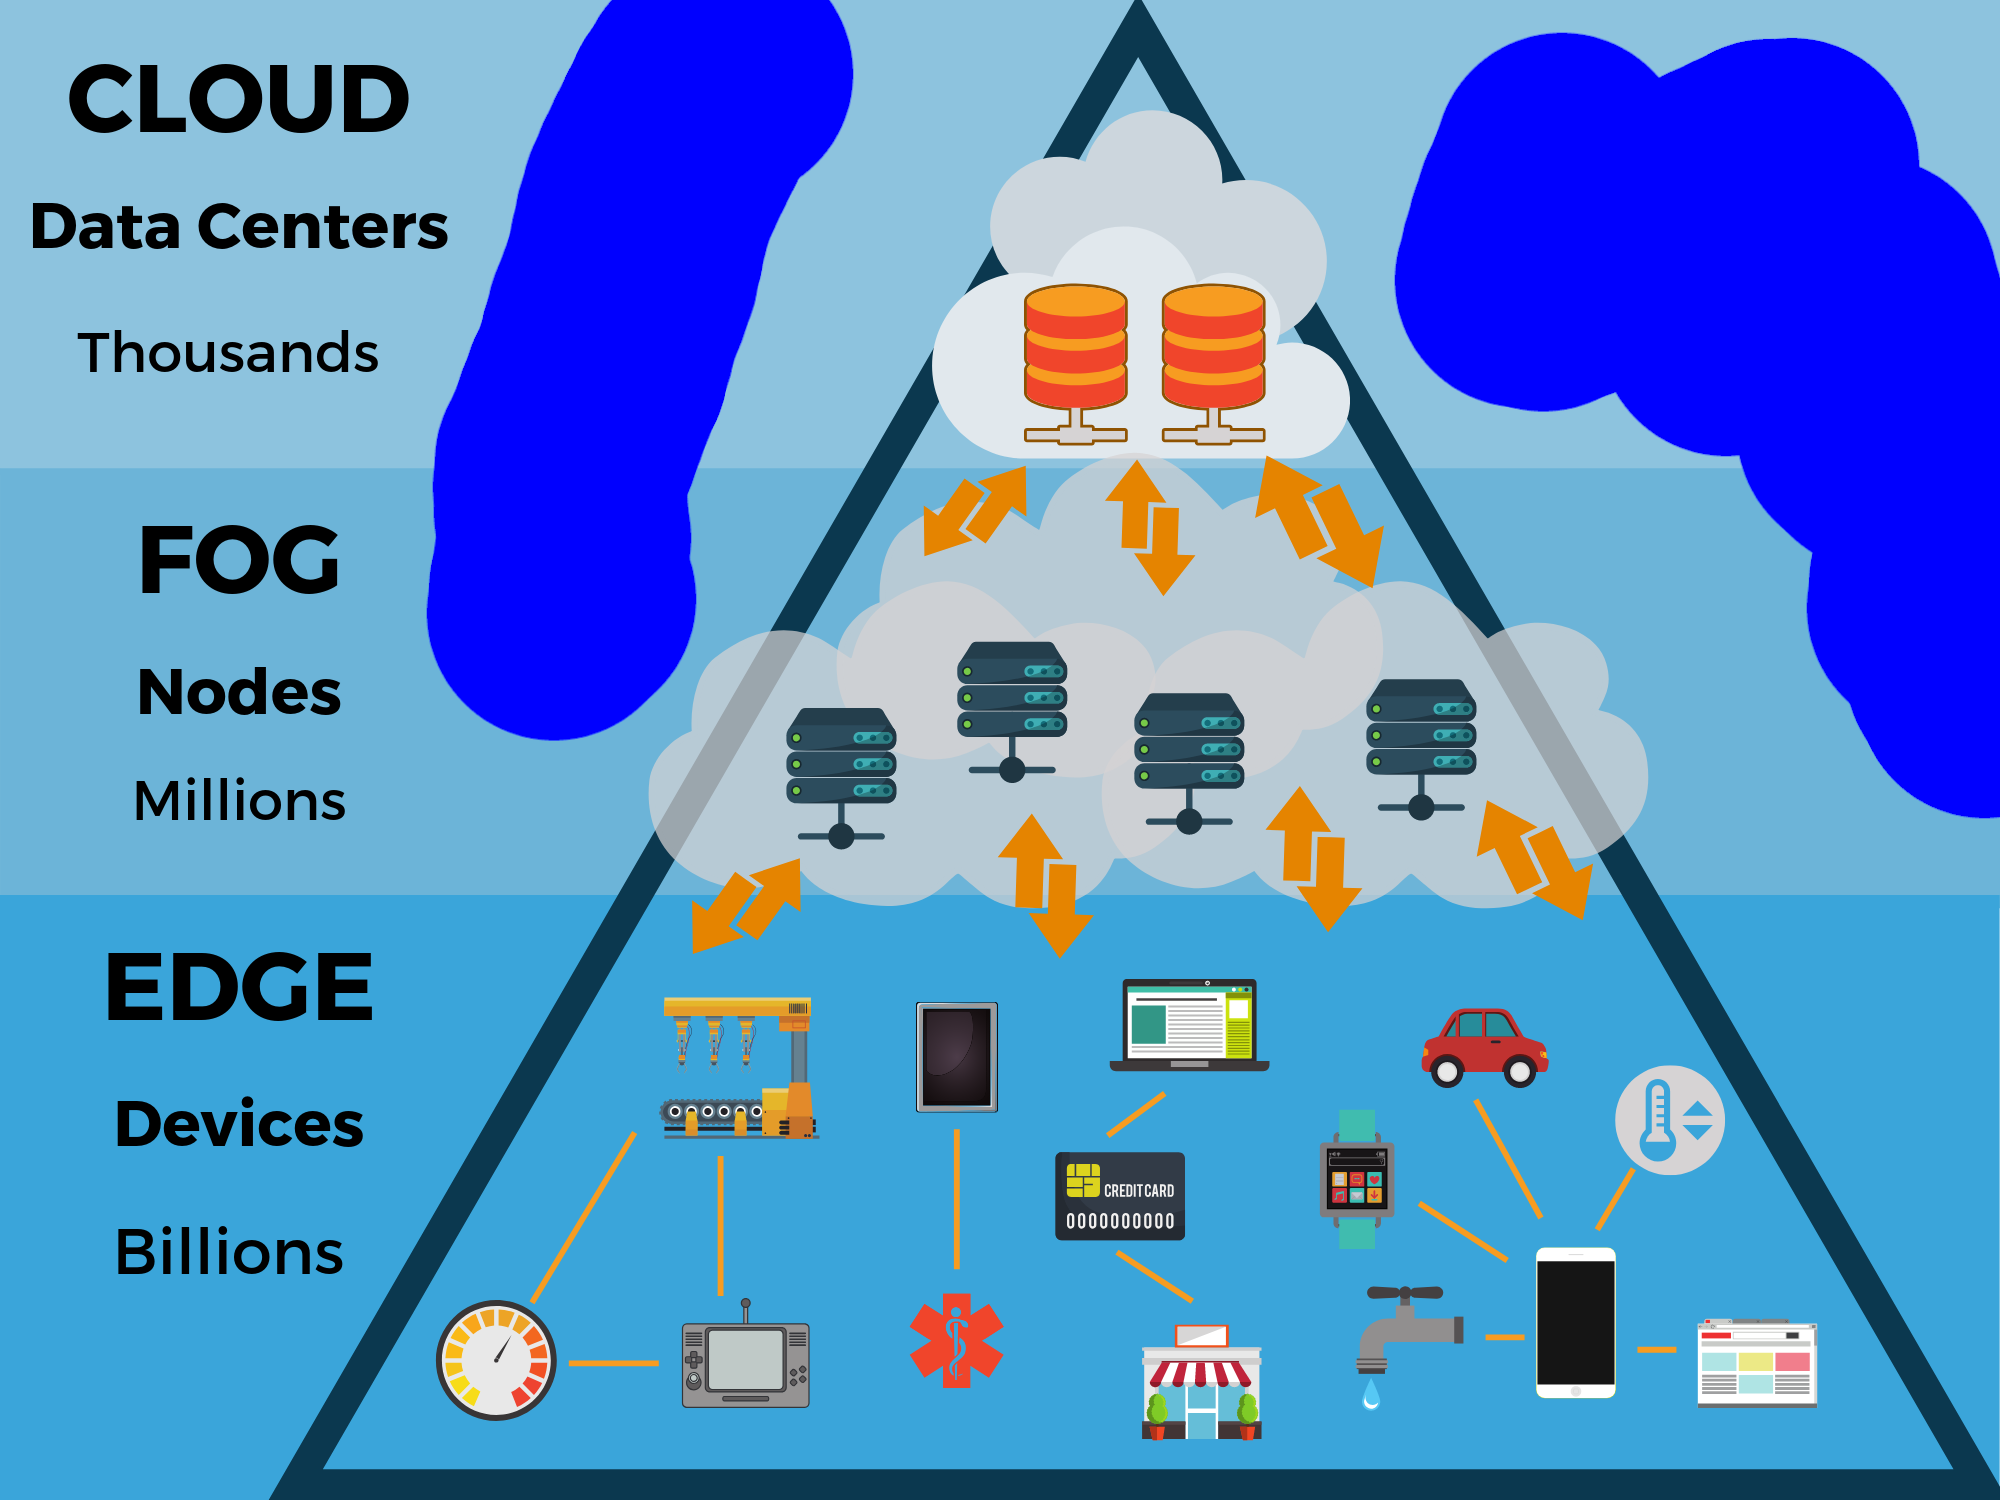
\includegraphics[width=\textwidth]{resources/img/chap2/computing_paradigms}
				\caption{Edge, Fog and Cloud Computing}
				\label{computing_paradigms}
			\end{figure}
		
			Each of these paradigms places computation on a different network layer, from Cloud Computing which lifts off all the need for end devices to compute data, to Edge Computing, where there might be specialized servers physically placed in strategic points so that they are closer to the end devices (lower latency), which may even have the ability to compute data by themselves.
			%https://www.cisco.com/c/en/us/solutions/computing/what-is-edge-computing.html
			On the other hand, Fog Computing is less aggressive than Edge Computing, and does not require the same amount of services placed near the clients, but they can be sorted among the backbone of the network.
			
			These communications do not take place only via Wi-Fi or Ethernet: given that ``\textit{things}'' can be everywhere, the need for a network that can adapt to a fast paced environment is becoming a must.
			Here is where the $5^{th}$ generation of cellular connectivity comes into play.
			
			%https://www.gsma.com/iot/resources/iot-5g-ltem-nbiot-opportunities-benefits/
			As described in a 2019 whitepaper by the GSM Association on IoT and the use of 5G, a ``\textit{combination of 5G and wireless edge technologies will support demanding  use cases, such as autonomous driving, time-critical industrial IoT manufacturing processes and  augmented and virtual reality (AR/VR)}'' \cite{IoT_5g_era}.
			Compared to what is possible with other transmission technologies, 5G supports a massive number in connections, with very little latency.
				
			All of this is not only interesting from a research point of view, but also from a market point of view, where new devices, for consumer and industrial purposes, are created to suit every possible need, that is why IoT can be considered as the ``\textit{next chapter of digital communication}''.
			
			The most notable example from a consumer's point of view, is the smartwatch, which started with the infamous Pebble watch\footnote{ \url{www.kickstarter.com/profile/getpebble/created}}, and is now considered almost a ``\textit{must-have}'' extension of the smartphone.
			Not only it smartwatches can be used for recreational purposes, but some models are crossing the line to becoming medical devices, given the improving accuracy with which they record data.
			Data that, in conjunction with AI, can be used to predict heart attacks \cite{7946780} or other diseases, like Hyperkalemia \cite{HYPERKALEMIA}.
			At the time of writing, IoT devices and frameworks can be used for contact tracing in order to prevent the spread of Covid-19 \cite{9181512}.
			
			Consumers want remote control of simple household devices such as coffee pots so that they may wake up to freshly	brewed coffee, or schedule it to be prepared at a given time.
			% \footnote{ \textit{Hyper Text Coffee Pot Control Protocol}: \url{www.datatracker.ietf.org/doc/html/rfc2324}}.
			
			On the other hand, from an industrial point of view, demands are more focused on fast connectivity among devices, ``\textit{Machine to Machine}'' (M2M), to constantly improve production of goods and services in Industry 4.0 and with the use of Industrial IoT (IIoT).
			% https://www.siemens-advanta.com/blog/what-are-expected-iot-trends-2021
			% IoT is an enabler for the sciences that need large amount of data for creating algorithms and offering better services and more well tailored products.
			The more data available, the more there are opportunities for science, services, business etc. to understand and improve and offer better services and more well tailored products.
			% https://www.mdpi.com/1999-5903/12/3/46
			The growing popularity of IoT use cases in domains that rely on connectivity spanning large areas and the ability to handle a massive number of connections is driving the demand for Low-Power Wide-Area-Network (LPWAN) access technologies, that is why the goal of fifth-generation (5G) wireless networks and beyond is to realize connecting ``\textit{anything, anyone, anytime, anywhere}'' \cite{7414384}.
			LPWANs are better explained in Section \ref{sec:radio_tech}.
			
			Given the importance of this economic sector, many companies, have analyzed the trends and have been producing forecasts about the growth of IoT.
			One analysis, made by The Economist's Intelligence Unit, and sponsored by Arm\footnote{ \url{www.arm.com}}, states that ``\textit{more than two-thirds of respondents agree that understanding the value of data helps them articulate the business case for IoT investments}'' \cite{economist-iot-business-index-2020-arm}.
			In the same analysis, IoT has emerged as an enabler for AI, since many companies ``\textit{view IoT and AI as two components of an advanced analytics capability}'', as previously mentioned.
	
			Underlying hardware challenges such as battery development and energy retention and consumption are among the main research areas that are being investigated, since they represent challenges to the realization of efficient IoT systems.
				
	\section{Air quality sensing}
	
		The ubiquity of mobile technology has opened the door to a new era of mobile sensing. 
		Through this new paradigm that is IoT, physical phenomena can be observed in a distributed way, crowd-sourcing data measurement tasks to smartphones and/or other popular smart wearables.
		Mobile sensing and wireless communications can hence be employed to gather data and generate new information and services, benefitting society.
		Two general strategies can be used to deploy an environmental monitoring system: creating a network of \textit{fixed sensors}	or resorting to \textit{mobile sensors}.
			
		The presence of tiny particulate matter in air is a crucial factor in health, especially when considering urban scenarios.
		In this context, smart mobility coupled with low-cost sensors can create a distributed and sustainable platform for social sensing able to provide pervasive data to citizens and public administrations. 
		Sustainable and eco-aware decisions can then be supported by empirical evidence, resulting in an improved life and better city administration.
		
		Some of the most harmful airborne agents are fine particles (PM2.5), sulphur dioxide (SO2), nitrogen dioxide (NO2), PM10, carbon monoxide (CO), benzene and ozone.
		The maximum amount for these particulates is regulated by various local and international authorities, for example the EU has set standards\footnote{ \url{www.ec.europa.eu/environment/air/quality/standards.htm}} that are reinforced by constant monitoring.
				
		One of the most important instruments in air quality measurement is the \textit{Keeling Curve}: a meticulous record of the amount of carbon dioxide in the atmosphere.
	
		\noindent
		\begin{minipage}{0.49\textwidth}%
			\begin{figure}[H]
				\centering
				\includegraphics[width=\textwidth]{resources/img/chap2/keeling}
				\caption{Full record Keeling curve until Nov. 1 2021}
				\label{keeling_full}
			\end{figure}
		\end{minipage}%
		\hfill%
		\begin{minipage}{0.49\textwidth}\raggedright
			\begin{figure}[H]
				\centering				
				\includegraphics[width=\textwidth]{resources/img/chap2/mlo_two_years}
				\caption{Two years Keeling curve until Nov. 2021}
				\label{keeling_two}
			\end{figure}
		\end{minipage}
		\newline
		
		The Keeling Curve tracks changes in the concentration of CO2 in the Earth's atmosphere using data from a research station on Mauna Loa, Hawaii.
		Figure~\ref{keeling_full} shows the result of daily readings that have continued almost uninterrupted for more than 60 years, while Figure~\ref{keeling_two} shows the data between October 2019 and November 2021.
		The importance of this instrument lies in the fact that, over those six decades, the zig-zag has trended steadily upward. 
		Real time readings can be found on the UC San Diego, Institution of Oceanography's dedicated website\footnote{ \url{keelingcurve.ucsd.edu}}.
		
		\textbf{\textcolor{red}{\hl{// To be completed, add research on low cost outdoor air quality sensors}}}
		
%		\cite{unknown}
%		LOW-COST OUTDOOR AIR QUALITY MONITORING AND SENSOR CALIBRATION: A SURVEY AND CRITICAL ANALYSIS
		
		Many projects have been made, both for research and commercial purposes, to detect pollutants in the air and raise awareness of the conditions people are living in.
		Below are two research solutions that have been made for air quality sensing with low-cost sensors.
			
		\subsection{ArduECO}\label{subsec:ardueco}
			% https://www.hackster.io/news/nodemcu-based-ardueco-aims-to-track-global-air-quality-metrics-using-bike-sharing-fleets-75d50e169fc8
			% https://www.math.unipd.it/~cpalazzi/ArduECO/ArduECO%20IEEE%20Presentation%20FINAL.pdf
			% https://arxiv.org/pdf/2007.08305.pdf
			
			ArduECO is a wireless device based on an Arduino-like board, esp8266, capable of gathering data about air quality (and more with simple extensions) and sending them to the cloud, to be processed and displayed.

			This solution has been proposed in the paper ``\textit{Air Quality Control through Bike Sharing Fleets}''\cite{ardueco_paper}, presented at the 2020 IEEE Symposium on Computers and Communications.
			
			\begin{figure}[h]
				\centering
				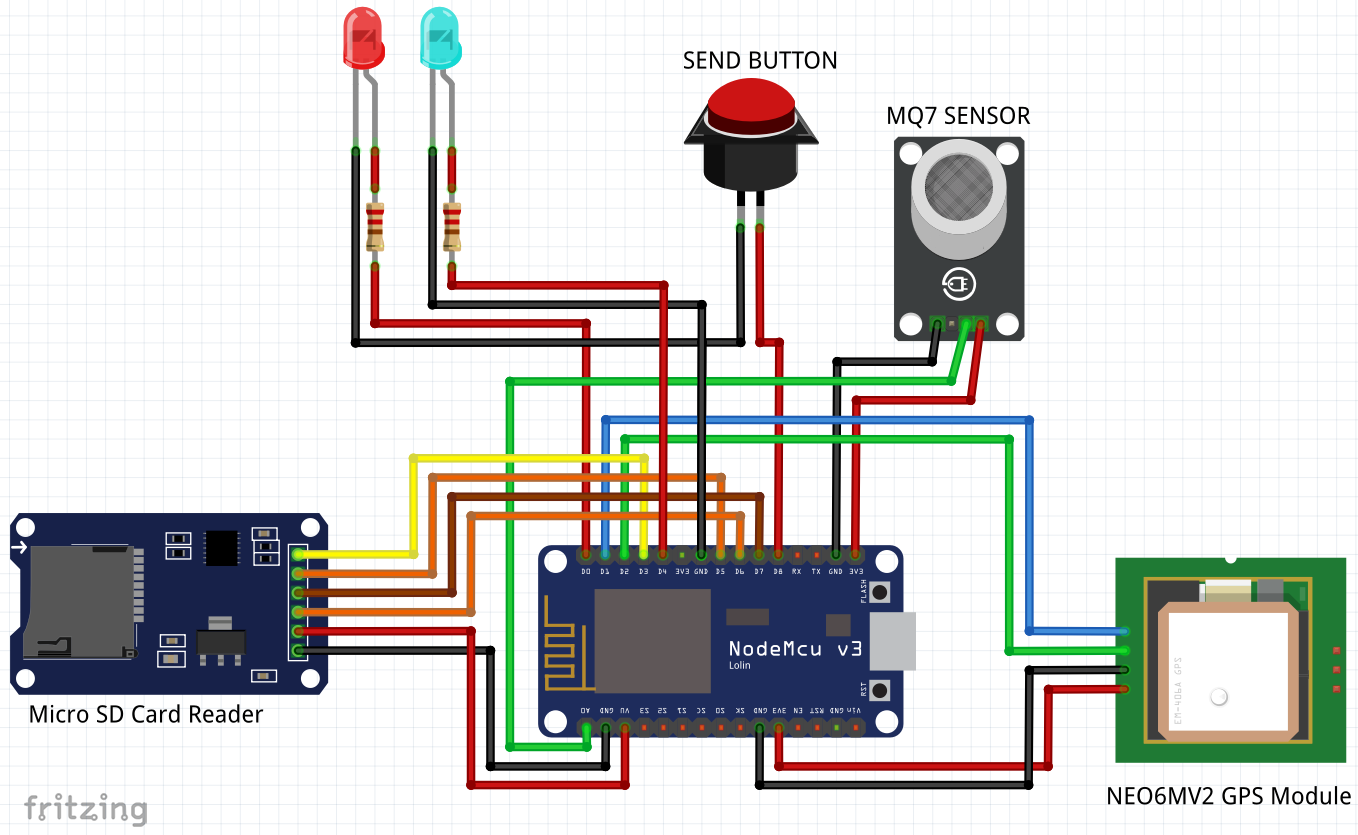
\includegraphics[width=.9\textwidth]{resources/img/chap2/ardueco_circuit}
				\caption{Circuit of the ArduECO prototype}
				\label{img:ardueco_circuit}
			\end{figure}
			
			One of the main design goals of this device is to be easily fit on shared means of transportation, such as bikes and electric scooters, which been advantaged by the COVID-19 pandemic \cite{HU2021102997}, contrast other shared transportation approaches, such as car sharing, that have severely suffered from the pandemic.
			
			ArduECO is built around four core components: the NodeMCU ESP8266-based development board, a microSD card reader for local data caching, a GPS-based global navigation satellite system receiver for location data and an MQ-7 carbon monoxide (CO) sensor, which can easily be replaced with other sensors using the same pinout.
			Figure~\ref{img:ardueco_circuit} shows the full circuit of the prototype, while Figure~\ref{img:ardueco_picture} is a picture of the built device.
			
			As well as capturing the air quality data locally, data is cached and later sent in the cloud to an MQTT server running on Amazon Web Services IoT Core.
			
			\noindent
			\begin{minipage}{0.38\textwidth}
				\begin{figure}[H]
					\centering
					\includegraphics[width=\textwidth]{resources/img/chap2/ardueco_picture}
					\caption{Built ArduECO prototype}
					\label{img:ardueco_picture}
				\end{figure}
			\end{minipage}%
			\hfill%
			\begin{minipage}{0.6\textwidth}\raggedright
				Server costs aside, the sensor platform can be built in a bill of materials of around $15$€, or less if the materials are bought in bulk.
				
				As described in the paper, this project is more of a proof of concept that shows the possibility of creating a small and cheap device which can be placed on shared means of transportation.
				Therefore there are various aspects that can be improved, such as adding multiple sensors to detect different pollutants and tweak the software so that the board can sleep and save battery.
			\end{minipage}

		\subsection{MegaSense}\label{subsec:megasense}
	
			% https://www.researchgate.net/profile/Samu-Varjonen
	
			% https://www.megasense.org/
			% https://uia-initiative.eu/en/uia-cities/helsinki	
			% https://ieeexplore.ieee.org/document/9248143
		
			MegaSense is a project that has been developed by the Departments of Computer Science at the University of Helsinki\footnote{ \url{www.helsinki.fi/en/computer-science}} and brings forward accurate portable low-cost sensing devices and an online data platform integrating multiple sources of urban data and leveraging AI network calibration producing hyper-local air quality information in real time.
				
			Compared to the previously described ArduECO, MegaSense, represented in Figure~\ref{img:megasense_picture}, is a more complete project which has been tested by citizens and companies in City of Helsinki and EU projects.
			It is also encased in a $3$D printed case and has an rechargeable battery, allowing it to be immediately given to the users.

			The back-end system receives data from sensing platforms, the individual MegaSense devices, measuring local pollution exposure and other variables affecting it.
			These data are processed into air quality information such as maps and advice on how to reduce personal exposure, take healthier routes, and direct participants to improve measurements in areas that have limited sensor coverage.
			
			\noindent
			\begin{minipage}{0.35\textwidth}
				\begin{figure}[H]
					\centering
					\includegraphics[width=.8\textwidth]{resources/img/chap2/megasense}
					\caption{MegaSense prototype}
					\label{img:megasense_picture}
				\end{figure}
			\end{minipage}%
			\hfill%
			\begin{minipage}{0.65\textwidth}\raggedright
				As explained in the main paper \cite{megasense} regarding this device, ``\textit{the core of MegaSense consists of two layers: the Edge and Cloud}''.
				The Edge layer receives data from available node and delivers pollution maps to the mobile app, which provides users with personal air pollution exposure	information as well as local exposure maps.
				This layer is responsible for data pre-processing, filtering and data cleaning.
				The cloud layer, which runs on AWS, is responsible for storing cleaned data	and aggregating the crowd-sourced data while preserving the privacy of participants.
			\end{minipage}
			\newline

			Registered citizens that have been given the device, download the HOPE Exposure App from Google play store and tether their Android smart phone to the sensor.
			The phone gathers data from the sensor, alongside the GPS coordinates, and it sends them in the cloud.


			\textbf{\textcolor{red}{\hl{// To be completed, add how calibration works + sensors}}}

%			\cite{8999428}		
%			Calibration Performance: We fi rst assess over-
%			all feasibility of calibration by assessing perfor-
%			mance of the mid-cost sensor after calibrating it
%			against a reference station. For calibration, we use
%			a deep learning model consisting of convolution-
%			al layers, fully connected neural network layers,
%			and long short-term memory (LSTM) layers that
%			model temporal dependencies.

%			\cite{megasense}
%			BME-280 Temp, Humidity, Air Pressure, 1
%			Battery Voltage 2
%			Sensirion SPS30 PM 3
%			SI1133-AA00-GM UV 4
%			MiCS-4514 CO, NO2 5
%			MQ-131 O3 6
			
			This project develops the clean air journey	planner application that creates optimal walking and cycling routes based on air quality of Helsinki.
			
			A better understanding of the architecture of MegaSense is explained in Section \ref{sec:architecture}, while the papers in which this project is detailed are \cite{8999428, megasense}. % Background
	%!TEX root = ../thesis.tex

\begin{savequote}[70mm]
	The Internet is becoming the town square for the global village of tomorrow.
	\qauthor{Bill Gates}
\end{savequote}


\chapter{Technologies}\label{chapter:technologies}
	
	This chapter explains more in detail the underlying technologies of this project.
	Starting from the general definition of a network and the most common architectures, to radio technologies work and then micro-controllers.
	
\section{Fundamentals of network communication}
	
	\begin{center}
		\begin{minipage}[H]{0.9\columnwidth}
			\begin{center}
				``\textit{A computer network is a structure that makes available to a data processing user at one place some data processing function or service performed at another place.}''~\cite{nla.cat-vn252493}
			\end{center}
		\end{minipage}
	\end{center}
	
	Starting from the definition of a computer network by Paul E. Green, it is easy to understand its importance in today's society.
	Smartphones, personal computers and other interconnected devices have become omnipresent in modern society, in which people need to feel connected to each other via these devices.
	% https://www.irishtimes.com/business/online-services-playing-more-important-role-in-everyday-activities-1.511857
	Not only they are used for fun, leisure and other social activities, but they allow connection to services such as online banking, government services and healthcare, that require a stable and secure connection among the systems that they use in order to provide a safe and sound experience for their users.
	All this to say, networks are everywhere underneath today's technology.
	There are no services or devices that can stand on their own without sharing data to other devices, to synchronize and provide a better user experience, to get updates from the manufacturer or simply to send a keep alive message.
	
	While this raw data is important for computers, people, the final users, process it to gain information, and this exchange of information from all around the world has brought radical changes many levels, from a cultural point of view to an economic point of view.
	The possibility of having a network of information exchange is the next step of globalization, which started with the exchange of goods among countries and now brings everyone together, allowing for a cultural exchange that lets people share and unite across the globe.
	
	This big network that is used to exchange information all around the world has a special name: Internet.
	% https://en.wikipedia.org/wiki/Right_to_Internet_access	
	% https://www.diplomacy.edu/blog/right-access-internet-countries-and-laws-proclaim-it/
	Many countries, such as Finland, Spain and Greece, have recognized the importance of this network and have given people the ''right to Internet access'', also known as the right to broadband or freedom to connect
	In these countries, service providers must be able to supply a mandatory minimum connection capability to all desiring home users in the regions of the country they serve.
	
	% http://www.redbooks.ibm.com/abstracts/gg243376.html
	It is important to note that Internet, with a capital I, is a particular set of worldwide interconnected networks \cite{gg243376}, but a common network of networks is called internetwork, shortened by internet, with a lowercase i.
	
	Such distinction began in the 1980s and has been described in RFCs \footnote{\href{https://datatracker.ietf.org/doc/html/rfc871}{RFC 871 (1982): A PERSPECTIVE ON THE ARPANET REFERENCE MODEL}}$^{,}$\footnote{\href{https://datatracker.ietf.org/doc/html/rfc872}{RFC 872 (1982): TCP-ON-A-LAN}} by computer scientists that understood how ARPANET was expanding and the its dimensions were not enough anymore to accommodate the amount of data traveling from one computer to another.
	% https://en.wikipedia.org/wiki/Commodore_64
	At that time, computers such as the IBM 5150 and the infamous Commodore 64 were starting to become more and more available, even if highly priced, not only to companies and universities, but also to consumers that brought them in their households, especially with the advent of MS-DOS, the dominant operating system throughout the 1980s and now open source \footnote{\url{https://github.com/microsoft/MS-DOS}}.
	
	As described by IBM in one of their technical books from the time, ''it is possible to divide the Internet such as the following groups of networks''\cite{gg243376}:
	\begin{itemize}[noitemsep]
		\item Backbones: large and strategical data routes among core networks and routers that compose and connect the Internet;
		\item Regional networks that connect large facilities such as universities and colleges;
		\item Commercial networks that provide to their subscribers access to the Internet;
		\item Local networks which run, for example, across a campus university;
	\end{itemize}

	% TODO sistemare posizione footnote alla fine
	% Oppure prendere mappa da https://www.globalbackbone.tisparkle.com/
	% Mettere riferimento a mappa interattiva
	% https://globe.gl/example/submarine-cables/
	\begin{figure}
		\centering
		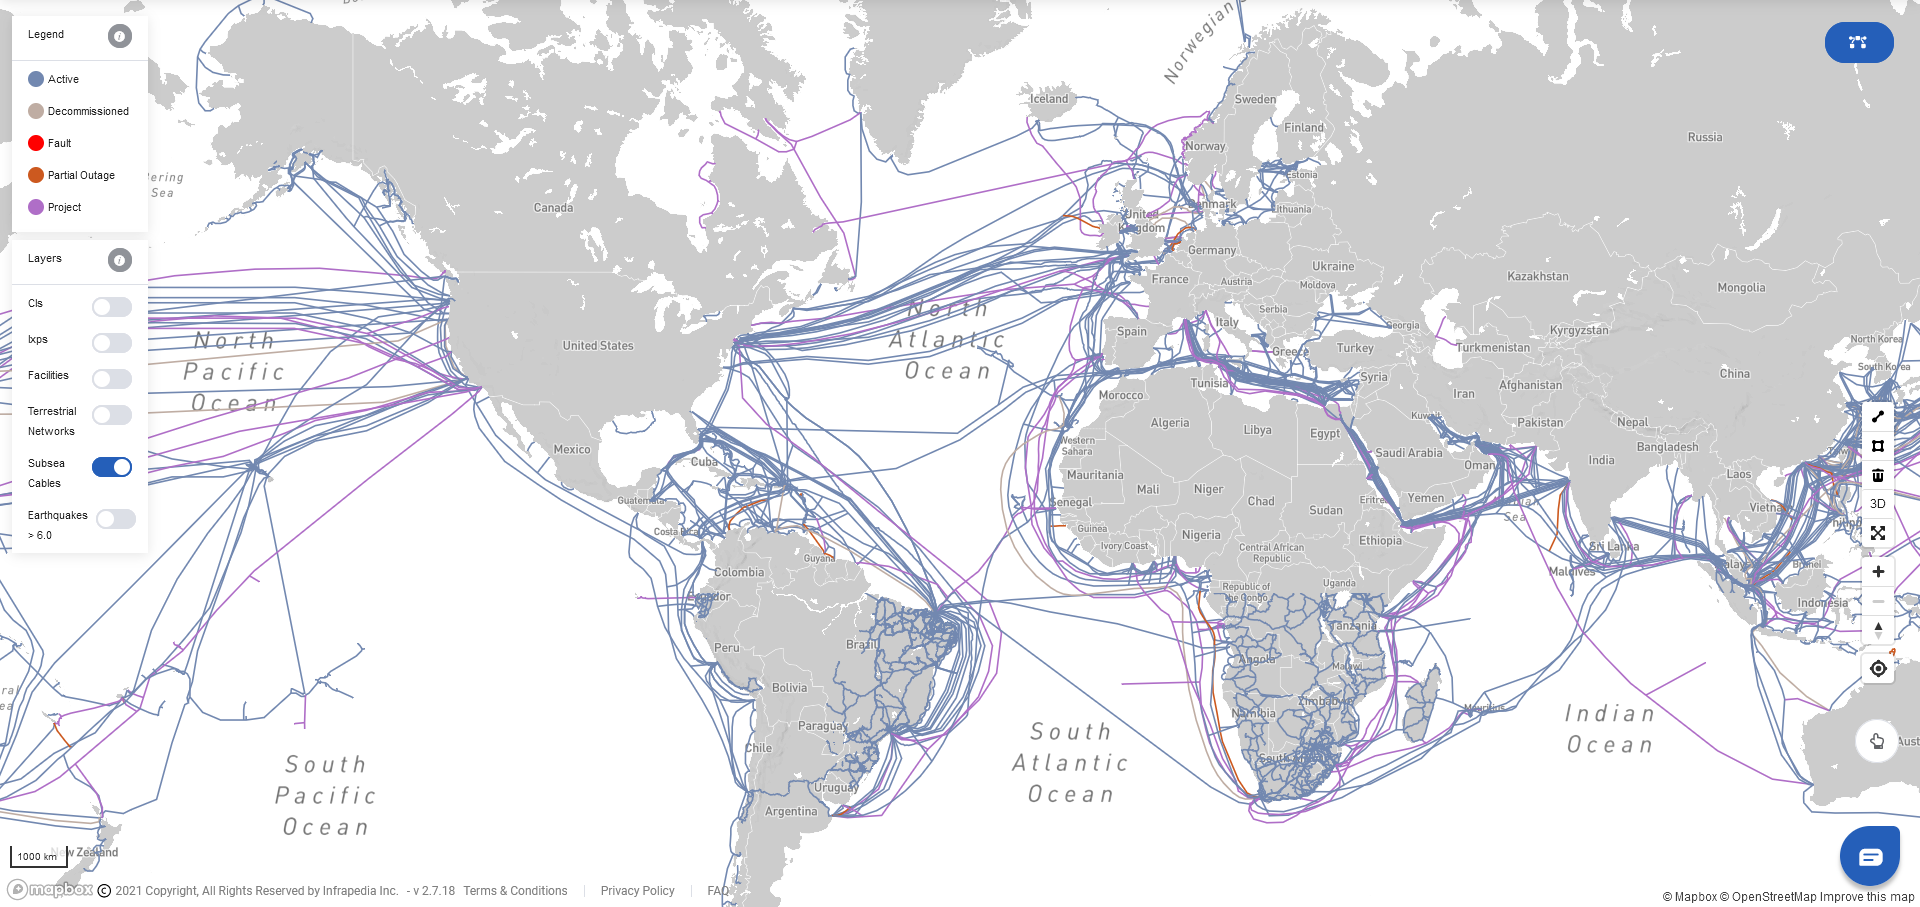
\includegraphics[width=\textwidth]{resources/img/chap3/backbone}
		\caption[Subsea Internet backbone cables between US and Europe.]{Subsea Internet backbone cables between US and Europe. \footnotemark}
	\end{figure}
	\footnotetext{~\url{https://www.infrapedia.com/app}}

	Given this increase of computers connecting to the Internet, there came the need for a revised structure that could better organize these components in a more robust, but also flexible, large network.

	With more accessible OSs, such as Windows 95 and Windows 98, and the advent of Tim Berners-Lee's World Wide Web (or WWW), computers became a commodity present in many households.
	The invention of the web and its ease to navigate, using hyperlinks and search engines, culminated in the dot com bubble, a stock market bubble in the late 90s that caused rapid rise of technology companies in stock market.
	
	Networks can be categorized based on the area they cover and serve:
	\begin{itemize}[noitemsep]
		\item Wide Area Network, or WAN: sometimes called long haul networks, provide communication over long distances;
		% https://www.cloudflare.com/learning/network-layer/what-is-a-metropolitan-area-network/
		\item Metropolitan Area Network, or MAN: provide communication inside a metropolitan area, which could be a single large city, multiple cities, or any given large area with multiple buildings;
		\item Local Area Network, or LAN: provide the highest speed connections among computers in a small and circumscribed area;
		% https://www.cloudflare.com/learning/network-layer/what-is-a-personal-area-network/
		\item Personal Ara Network, or PAN: connects devices within a user's immediate area.
	\end{itemize}

	In Sec. \ref{sec:radio_tech}, is described another level of distinction based on the power consumed by the transmission medium.
	
	Since everyone can connect to the Internet and access it's services, there is no need for the average user to understand what happens between his machine and the rest of the network, which means he only sees the information that is displayed to him without knowing where it arrives from or what path it took to arrive on his monitor.
	
	% inserire immagine con la nuvoletta che si vede dentro e non si vede dentro ?
	
	For computer scientists though, it is important to understand the difference between network architecture and network topology.	
	A network architecture, as described by by Paul E. Green, ``is a complete definition of all the layers necessary to build the network''\cite{nla.cat-vn252493}.
	This is focused on the network software, which needs to be highly structure in order to allow for heterogeneous systems to communicate with each other.
	% https://standards.iso.org/ittf/PubliclyAvailableStandards/s020269_ISO_IEC_7498-1_1994(E).zip
	One example of network architecture is the ISO/OSI reference model \footnote{\url{https://www.iso.org/standard/20269.html}}, which is implemented by the TCP/IP stack of protocols.
	
	% https://stackoverflow.com/questions/38596488/in-which-layer-is-http-in-the-osi-model
	\begin{figure}[H]
		\centering
		\includegraphics[width=\textwidth]{resources/img/chap3/isoosi}
		\caption{The ISO/OSI reference model against the TCP/IP stack}
	\end{figure}
	
	Thus comes the definition of a protocol as ``a set of agreements for interaction of two or more parties and is expressed by three components, syntax (e.g., a set of headers, a set of commands/responses), semantics (the actions and reactions that take place, including the exchange of messages), and timing, the sequencing and concurrency aspects of the protocol.''\cite{nla.cat-vn252493}.
	% TODO rivedere contenuto tra parentesi
	Different types of network use different architectures, based on the transmission medium and how well this performs (errors, speed, etc.).
	
	% https://www.omnisci.com/technical-glossary/network-topology
	On the other hand, the network topology refers to the manner in which the links and nodes of a network are arranged to relate to each other.
	
	\begin{figure}[H]
		\centering
		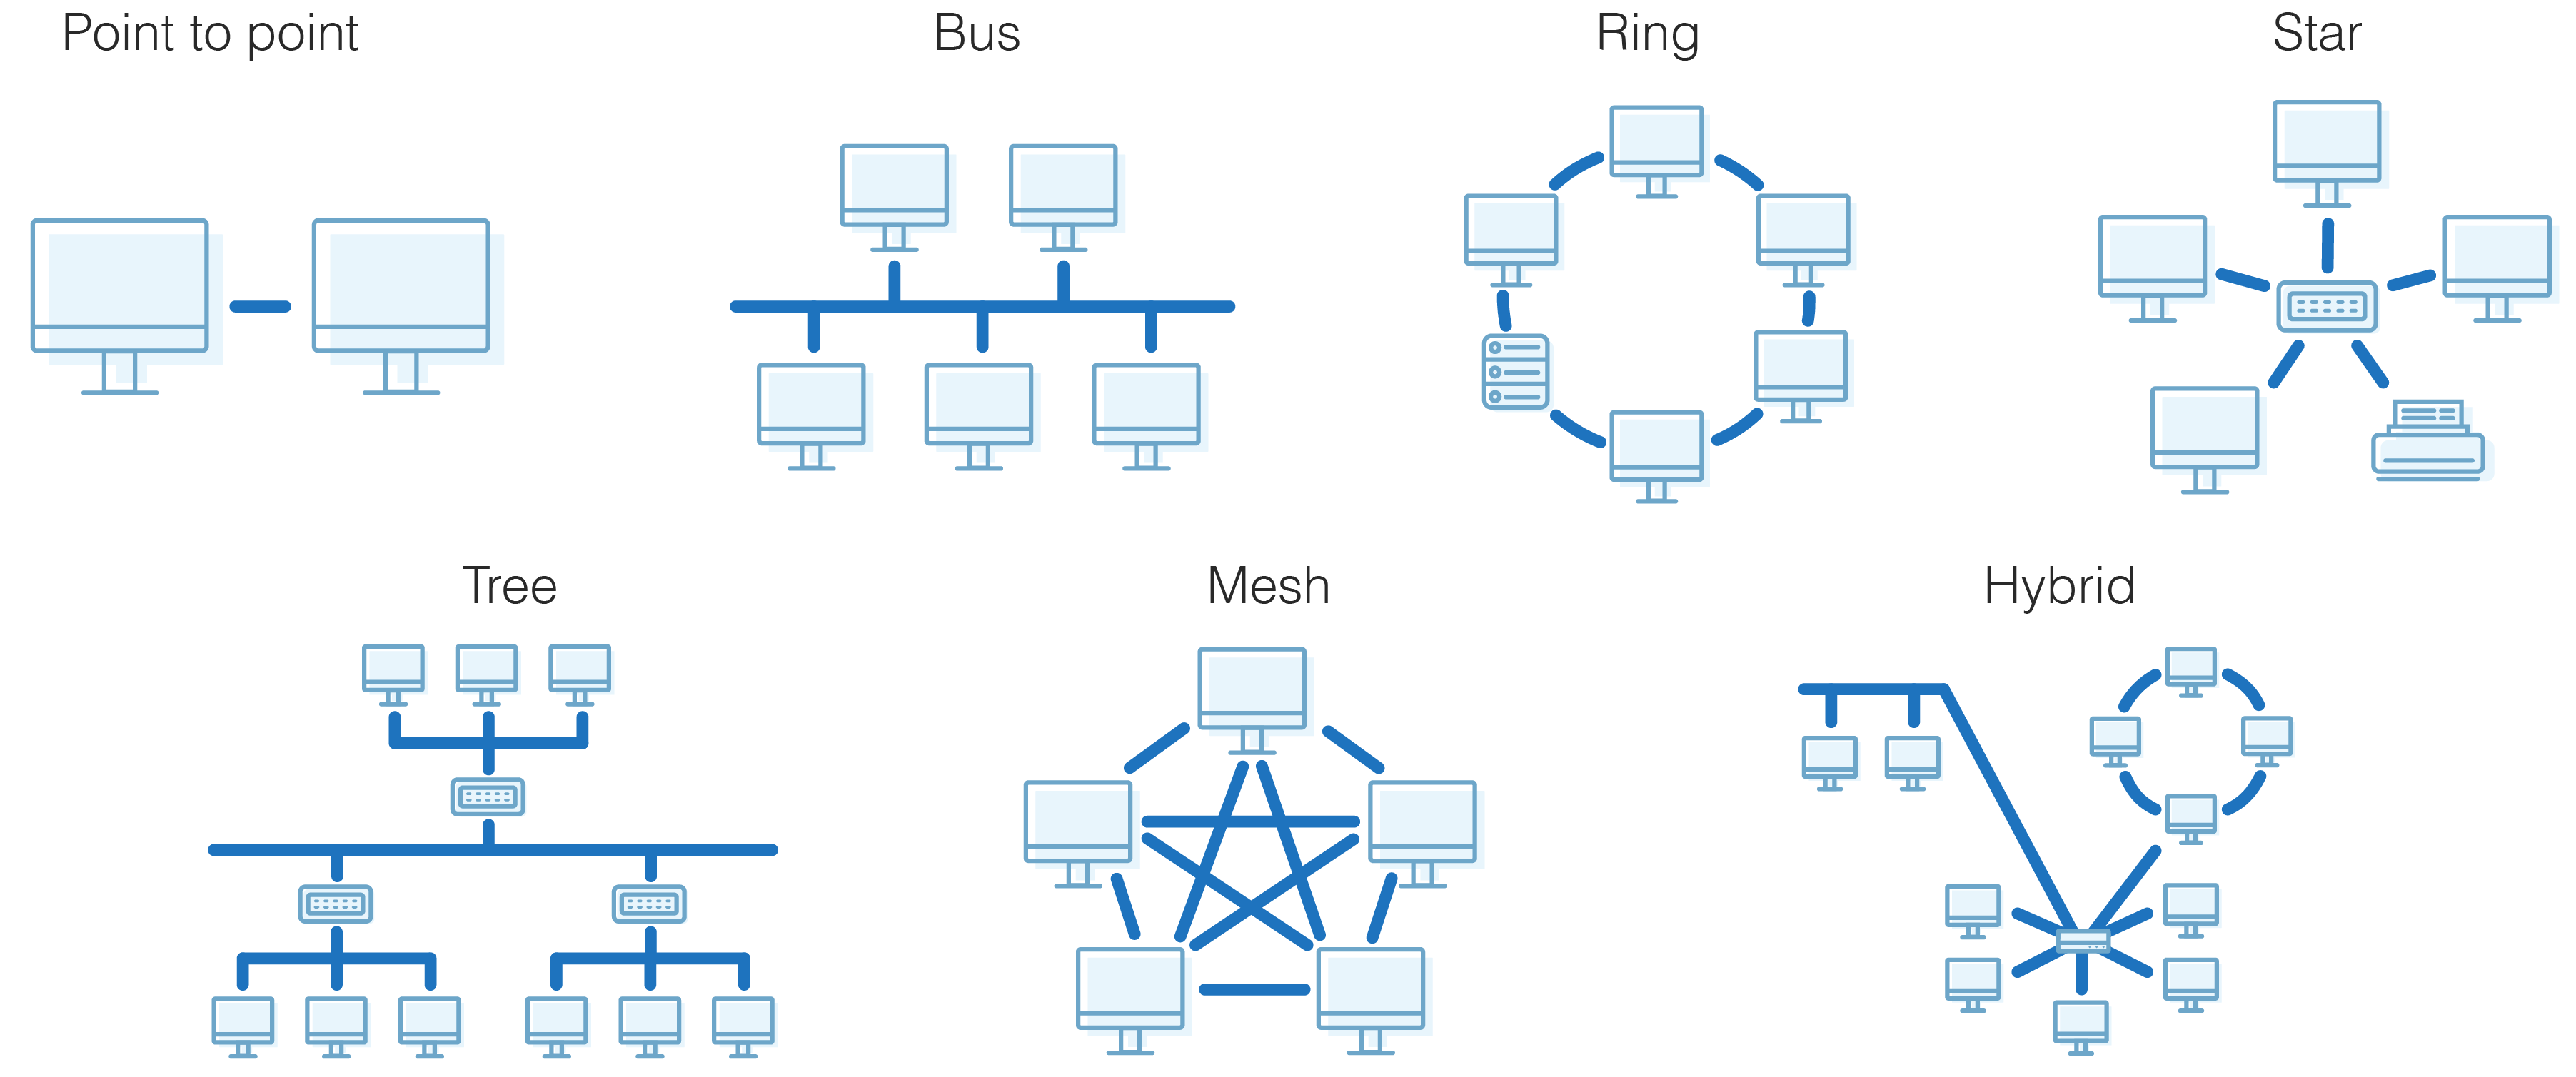
\includegraphics[width=\textwidth]{resources/img/chap3/network_topologies.png}
		\caption{Common network topologies}
		\label{img:network_topologies}
	\end{figure}
	
	As shown in Fig. \ref{img:network_topologies}, some of the most common network topologies are:
	\begin{itemize}[noitemsep]
		\item Point-to-Point: in which devices are connected directly;
		\item Bus: devices are connected to each other via a backbone cable;
		\item Ring: two dedicated point-to-point links connect a device to the two devices located on either side of it, creating a ring of devices through which data is forwarded via repeaters until it reaches the target device;
		\item Star: connects each device in the network to a central hub. Devices can only communicate with each other indirectly through the central hub;
		\item Tree: parent-child hierarchy in which star networks are interconnected via bus networks;
		\item Mesh: a dedicated point-to-point link connects each device on the network to another device on the network, only carrying data between two device;
		\item Hybrid: any combination of two or more topologies;
	\end{itemize}

	% TODO rivedere bene quando si scrive resto della tesi
	The project presented in this thesis regards a network with a mesh topology.
	This is better described in chap5 in a more depth and technical way
	The mesh proposed in this thesis has a span of LAN / MAN, since it connects devices that are in a circumscribed area but can be also placed further from each other, in order to cover longer distances.
	
	% TODO è necessaria?
	Another important distinction to make is the one between a distributed systems and a computer network.
	
	% COPIATO DA INTERNET: responsible for technical management of IETF activities and the Internet standards process
	Nowadays, the organization responsible for technical management of IETF activities and the Internet standards process is the Internet Engineering Steering Group (IESG)\footnote{\url{https://www.ietf.org/about/groups/iesg/}}.
	It is necessary to have an organization looking over the Internet itself since it gives the regulations that allow all devices to interconnect with each other.

\section{Radio technologies}\label{sec:radio_tech}
	
	% https://en.wikipedia.org/wiki/Invention_of_radio
	Although Guglielmo Marconi is usually credited as the inventor of radio due, to the creation of the first commercially successful wireless communication system \cite{4137304}, many scientists before him have studied the subject of radio waves.
	The discovery of electromagnetic waves, including radio waves, by Heinrich Rudolf Hertz in the 1880s, came after theoretical development on the connection between electricity and magnetism that started in the early 1800s.
	Scientists tried to achieve the idea of a wireless telegraph via electric conduction and electromagnetic induction for a while before the establishment of radio-based communication.
	
	% https://science.howstuffworks.com/innovation/inventions/who-invented-the-radio.htm
	Other important experiments were made by Nikola Tesla, who invented the Tesla coil, a device essential to sending and receiving radio waves, during efforts to develop a "wireless" lighting system.
	% TODO aggiungere patent?
	This Tesla coil has been used by Marconi in his experiments and is present in the patent he presented for radio transmission of data.
	
	More than a century later, radio technology has massively evolved and is used on a daily basis.
	Devices has shrunk and the amount of transmission meanings have increased far from what both Tesla and Marconi could have thought of.
	Thus, in order to give a complete picture of radio transmitting technologies, it is important to make a distinction among the ones that are made for internal or nearby use vs the ones that are used for longer distances.
	
	% https://sites.google.com/site/pnutpck11/lesson-9---wireless-transmission-media
	Many users opt for wireless transmission media because it is more convenient than installing cables, even if they might sacrifice some performance. 
	Also, using wireless technology allows transmission in locations where it is impossible to install cables.
	% TODO RIVEDERE COPIATA SPUDORATAMENTE
	Types of wireless transmission media used in communications include infrared, broadcast radio, cellular radio, microwaves, and communications satellites.
	\begin{itemize}[noitemsep]
		\item Infrared: wireless transmission medium that sends signals using infrared light waves
		\item Broadcast Radio: wireless transmission medium that distributes radio signals through the air over long distances such as between cities, regions, and countries and short distances such as within an office or home. Bluetooth, UWB, Wi-Fi, and WiMAX communications technologies use broadcast radio signals.
		\item Cellular Radio: form of broadcast radio that is used widely for mobile communications, specifically wireless modems and cell phones, which use high-frequency radio waves to transmit voice and digital data messages.
		\item Communications satellite: space station that receives microwave signals from an earth-based station, amplifies (strengthens) the signals, and broadcasts the signals back over a wide area to any number of earth-based stations.
		Applications such as air navigation, television and radio broadcasts, weather forecasting, video conferencing, paging, global positioning systems, and Internet connections use communications satellites.
	\end{itemize}
	
	With new transmission technologies, new network architectures and topologies that are better suited for the transmission method have emerged.
	Topologies that bring computation closer to the edge are also rising in popularity, since they allow for faster computation and they bring data closer to the user.
	
	LAN MAN and WAN are not enough anymore to describe the new topologies.
	An important distinction is now made by other factors such as power consumption, cost of the devices and range of the transmiter and receiver.
	
	The most important new category of wireless communication, that interests IoT and reprents a large portion of the market at the time of writing, as described in chap2, is LPWAN, which stands for Low Power Wide Area Networks.
	
	The characteristics of LPWAN are: long range, low power and low cost.
	% https://en.wikipedia.org/wiki/Low-power_wide-area_network
	Lightweight protocols reduce complexity in hardware design and lower device costs. Its long range combined with a star topology reduce expensive infrastructure requirements, and the use of license-free or licensed bands reduce network costs.

	% http://iotfactory.eu/iot-knowledge-center/overview-of-iot-networks/	
	% TODO CAMBIARE E CITARE
	% https://www.mdpi.com/1999-5903/12/3/46
	The growing popularity of IoT use cases in domains that rely on connectivity spanning large areas and the ability to handle a massive number of connections is driving the demand for LPWAN access technologies \cite{fi12030046}, and the project presented in this thesis falls under this category of communication.
	LPWAN allows connectivity in many applications, from crowded areas in smart cities to smart farming and smart environment, from security and emergencies to e-health.
	
	Various wireless transmission methods can be used to create a LPWAN, some of the most used in IoT are Sigfox, LoRa and NarrowBand IoT (NB-IoT).
	In subsection \ref{subsec:lora_lorawan}, follows a more complete explanation on LoRa and LoRaWAN.
	One important factor for all these transmission methods is to support a massive number of simultaneously connected devices with low data rates \cite{fi12030046}.
	
	Other important communication technologies in IoT are RFID, NFC, for contact purposes, Bluetooth, Zigbee for a personal network and IEEE 802.11, or WiFi, for a local area.
	The latter was used in the ArduEco project, described in chap2.
	Fig. \ref{img:wireless_coverage} contains a representation of the geographic coverage in meters of the various aforementioned wireless transmission methods.

	
	% TODO sistemare posizionamento immagine
	% \newpage
	\begin{figure}
		\centering
		\includegraphics[width=\textheight,height=\textwidth,keepaspectratio,angle=90]{resources/img/iot_range}
		% \includegraphics[height=\textwidth, angle=90]{resources/img/iot_range}
		\caption[Wireless access geographic coverage.]{Wireless access geographic coverage. \cite{fi12030046}}
		\label{img:wireless_coverage}
	\end{figure}
	% \newpage

	\subsection{LoRa and LoRaWAN}\label{subsec:lora_lorawan}
	
		% TODO modificare perchè copiato spudoratamente
		% https://www.semtech.com/lora
		LoRa (short for long range) is a spread spectrum modulation technique derived from chirp spread spectrum (CSS) technology.
		Semtech’s LoRa is a long range, low power wireless platform that has become the de facto wireless platform of Internet of Things (IoT).
		
		% https://www.design-reuse.com/news/28706/semtech-cycleo-acquisition.html
		% https://blog.semtech.com/a-brief-history-of-lora-three-inventors-share-their-personal-story-at-the-things-conference
		Since it's development in 2009, by the french company Cycleo, now acquired by the semiconductor company Semtech, LoRa has come a long way.				
		On top of it, there is a proprietary MAC protocol called “LoRaMAC”, which specifies the message formats and security layers for a true networking protocol.
		
		In February 2015, the LoRa Alliance was founded and the networking protocol was renamed “LoRaWAN.”
		% https://lora-alliance.org/
		The LoRa Alliance is a non-profit organization committed to enabling large-scale deployment of Low Power Wide Area Networks (LPWAN) IoT through the development and promotion of the LoRaWAN open standard.
		
		This organization is alike with the 3GPP 
		
		Applications of LoRa in IoT varies from smart agriculture, to smart cities, to contact tracing, to logistics and healthcare.
		A complete list of the whitepapers on LoRa based communication can be found on Semtech's official website \footnote{\url{https://www.semtech.com/lora/lora-applications}}.
		
		% TODO aggiungere tabella con specifiche
		
		\begin{figure}[H]
			\centering
			\includegraphics[width=\textwidth]{resources/img/LoRa_Why_Range}
			\caption{}
		\end{figure}

%		The smaller the package, the greater the range.
%		The greater the range, the fewer receiving antennas.
%		The fewer antennas, the lower the total costs for the user.

\section{Hardware (Microcontrollers)}\label{sec:microcontrollers}

	Microcontrollers (or MCUs, short for Microcontroller Unit) are compact integrated circuits designed to govern a specific operation in an embedded system.
	They are specially made to fit in particular environments or to perform specific functions, which usually do not require any particular computation, memory capacity or power.
	This has been made possible thanks to the continuous shrinking of transistors, which makes almost all the components more compact, and the improved power sources.
	% TODO cambiare batteries con qualcos'altro?
	In junction with the previously described wireless technologies, microcontrollers are at the hearth of IoT devices, described in Chap. \ref{chap:background}, and they require long-lasting, low-cost, and sustainable batteries.
	
	% TODO modificare un attimo
	% TODO da riprendere in chap2
	% https://ieeexplore.ieee.org/abstract/document/9148855?casa_token=ppFhpgagThgAAAAA:u81u3jhRB-EJxsnQFx32i8LI4nJBKi3NsDvemcunZKNeSETGloW8wRB45S5OeaYOOdh2kXQ
	The number of IoT connected devices is expected to grow up to 75 billion worldwide by 2025 \cite{statista}, and connection density is expected to be one million devices per square km\cite{noma}.
	These devices will generate massive data and consume significant energy.
	
	Given the amount of specific functions an MCU can perform, there are many boards on the market.
	Some are very alike, while others are very different, since they are expected to be used in other types of environments.
	All boards consist on a similar architecture, which contains the processing unit (CPU), along with memory and programmable input/output peripherals.
	
	\begin{figure}[H]
		\centering
		\includegraphics[width=\textwidth]{resources/img/chap3/generic_board}
		\caption{Attiny 85 on the left, in the middle two boards based on the ESP32, on the right the Asus Tinkerboard 2}
		\label{img:generic_board}
	\end{figure}

	% https://en.wikipedia.org/wiki/Microcontroller
	In Fig. \ref{img:generic_board}, there are four different boards, the one farthest on the left is the ATtiny 85 \footnote{\url{https://www.microchip.com/en-us/product/ATTINY85}}, a low-power, 8-bit microcontroller that is made for general purpose and can be programmed for simple tasks, from simple LEDs flashing, to more elaborate small sensor projects.
	% https://en.wikipedia.org/wiki/ESP32
	The two boards in the middle are based on the ESP32 chip, a series of low-cost, low-power system on a chip microcontrollers with integrated Wi-Fi and dual-mode Bluetooth.
	They both are more powerful than the ATtiny 85, and right one offers an integrated LoRa antenna on board.
	Far on the right, there is the Asus Tinkerboard 2 \footnote{\url{https://tinker-board.asus.com/product/tinker-board-2.html}}, a board powered by an Arm 6-core system on a chip (SoC), with a 64-bit Armv8 architecture.
	This board provides much more computing power compared to the previous ones and is able to run operating systems such as Linux and Windows.
	
	% https://www.amazon.it/Meipai-ATTINY85-20PU-ATTINY85-chip-ATMEL/dp/B08HPPMJ52/
	% https://www.amazon.it/AZDelivery-NodeMCU-Development-Arduino-gratuito/dp/B071P98VTG/
	% https://www.amazon.it/Scheda-Modulo-Wireless-T-Beam-Batteria/dp/B07X2KPN4L/
	% https://www.welectron.com/navi.php?qs=Tinker
	One of the strong points of these boards is the price: the ATtiny is priced around 1€ when bought in bulk, the boards on the middle cost around 7€ and 15€, while the board by Asus is the more expensive and starts from 70€.
	
	It is important to note though that using a generic board in a production environment might not be ideal, since it might lack of support and documentation.
	The boards described subsequently are from three of the major MCU producers, Arduino, Raspberry Pi and Pycom, which have built hardware that is well documented and suited for many different environments, from hobbysts to industrial use.
	
	The simplified architectures and the constraints of embedded devices are reflected in the narrow choice for programming languages.
	It is hard to find an MCU programmed in Java since this would require the JVM running in the background.
	Popular languages for MCUs are, for example, C/C++, Assembly, Rust, Ada, Erlang, etc.
	% TODO CONTROLLARE
	All these have in common the fact that they are compiled and the bytecode has a small footprint.
	A particular microcontroller company, Arduino, have developed a version of C++ specific for their boards, but given the simplictity of this new dialect, many boards on the market can be programmed with it.
	Arduino is explained further in Subsection \ref{subsec:arduino}.

	% TODO da spostare in 
	Another programming language that is quickly taking hold at the time of writing, is Mycropython.
	As explained in their website it is an "efficient implementation of the Python 3 programming language that includes a small subset of the Python standard library and is optimised to run on microcontrollers and in constrained environments" \footnote{\url{https://micropython.org/}}.
	% https://itqna.net/questions/437/what-definition-verbose-code-and-why-it-interesting-reduce-i
	Python's fast learning and explicit code advantages are reflected in this smaller version for microcontrollers, available for most of them.
	
	Below is a table with the specifications of microcontrollers from Arduino, Raspberry Pi and Pycom, which are better described in the following subsections.
	\begin{table}[htbp]
		\begin{center}
			\begin{tabularx}{\textwidth}{@{}|Y|Y|Y|Y|Y|Y|@{}} 
				\hline
				& Arduino UNO R3 & Arduino Nano BLE & Raspberry Pi & Rasperry Pi Pico & Pycom FyPy \\\hline
					CPU &&&&& \\\hline
					RAM &&&&& \\\hline
					ROM &&&&& \\\hline
					IO PINS &&&&& \\\hline
					PORTS &&&&& \\\hline
			\end{tabularx}
			\caption{Specifications of Arduino, Raspberry Pi and Pycom microcontrollers}
			\label{table:1}
		\end{center}
	\end{table}

	\subsection{Arduino}\label{subsec:arduino}
	
		% https://www.arduino.cc/en/Main/AboutUs
		% https://www.oreilly.com/library/view/arduino-a-technical/9781491934319/ch01.html	
		Arduino is a company founded by Massimo Banzi Et Al. in Ivrea, Italy, in 2005, and has released the first commercially available microcontroller.
		% TODO rivedere
		They wanted a device that was simple, easy to connect to various ''things'' (such as relays, motors, and sensors), and easy to program, besides being inexpensive.
		% It also needed to be inexpensive, as students and artists aren’t known for having lots of spare cash. 
	
		They selected the AVR family of 8-bit microcontroller devices from Atmel and designed a self-contained circuit board with easy-to-use connections, wrote bootloader firmware for the microcontroller, and packaged it all into a simple integrated development environment (IDE) that used programs called “sketches”. 
		Arduino was the result.
		
		The most famous version of their board is the UNO (one in English).
		Arduino UNO, the one on the left in Fig. \ref{img:arduino_board}, is the most used and documented board of the whole Arduino family.
		% https://www.circuito.io/blog/arduino-uno-pinout/
		Although this board does not have any integrated sensors or particular ports for peripherals.
		The current revision of the board is the Arduino UNO Rev 3 \footnote{\url{https://store.arduino.cc/products/arduino-uno-rev3}}, which consists of 14 digital pins, 6 analog inputs, a power jack, USB connection and ICSP header.
		
		% https://store.arduino.cc/products/arduino-uno-rev3
		% https://store.arduino.cc/products/arduino-yun-rev-2
		% https://store.arduino.cc/products/arduino-nano-33-ble
		\begin{figure}[H]
			\centering
			\includegraphics[width=\textwidth]{resources/img/chap3/arduino_types}
			% TODO rivedere accento yun, mettere link?
			\caption{Arduino UNO Rev 3 on the left, Arduino Yun in the middle, Arduino Nano 33 BLE on the right}
			\label{img:arduino_board}
		\end{figure}
		
		% https://www.circuito.io/blog/arduino-code/
		The Arduino family of products can be programmed in a particular programming language based on C/C++, using a special open-source integrated development environment (IDE).
		Arduino was so disruptive in the market that many boards, included the ones in Fig. \ref{img:generic_board}, support the Arduino C++.

		Shields are modular circuit boards that can be added to extend capabilities to different application needs.
		These can be attached directly on top of the board and provide sensors, interfaces, peripherals on a single board, rather than attaching to the Arduino singularly.
		% https://learn.sparkfun.com/tutorials/arduino-shields
		Some of the functionalities that can be added by a shield are Ethernet, WiFi, GPS, displays and cameras, motor drivers.
		Most of the additional shields on the market have been developed for the Arduino UNO, since it is the most common board.
		
		The choice of making the Arduino schematics open-source and accessible to anyone has largely favored the development of newer boards, similar in capacity to the Arduino but more specialized, since producers and board makers are able to keep only the components needed or add different ones.
		An example can be the two middle boards in Fig. \ref{img:generic_board}, which rode the wave of Arduino's popularity.
		Not only the datasheets are available for all boards, but also the Arduino IDE software is open-source.
		
		% https://www.circuito.io/blog/arduino-code/
		The versatility of Arduino and its simple interface makes it a leading choice for a wide range of users around the world from hobbyists, designers, and artists to product prototypes. 
		
		Newer Arduino boards offer many integrated functionalities, for example:
		\begin{itemize}[noitemsep]
			% https://store.arduino.cc/collections/boards/products/arduino-mkr-nb-1500
			\item Arduino MKR NB 1500: offers an all-in-one solution for Narrowband IoT large-coverage solutions;
			% https://store.arduino.cc/collections/boards/products/arduino-mkr-wifi-1010
			\item Arduino MKR WiFi 1010: offers integrated WiFi and Bluetooth;
			% https://store.arduino.cc/collections/boards/products/arduino-nano-33-ble-sense
			\item Arduino Nano 33 BLE Sense: contains BLE connectivity and multiple sensors, such as 9 axis inertial, humidity, and temperature, barometric, microphone, gesture, proximity, light color and light intensity.
		\end{itemize}
	
		% TODO rivedere bene quando si scrive resto della tesi
		Particularly, this last model, the board on the right in Fig. \ref{img:arduino_board}, has been considered as one of the possible choices as development board for this project.
		As better explained in chap 5, it has been discarded since it does not offer LoRa connectivity and an additional module would have been necessary to connect the board in a mesh.
							
	\subsection{Raspberry Pi}

		% https://ccclib.org/raspberrypi/
		% https://www.electronicshub.org/raspberry-pi-vs-arduino/
		Another important microcontroller on the market is the Raspberry Pi, developed by Eben Upton at the University of Cambridge in the United Kingdom with the aim of teaching and improving programming skills of students in developing countries.
		
		Compared to the Arduino specifications, it also offers more functionalities, since they include an ARM processor, a GPU with HDMI output connectivity, an Ethernet port, USB ports to connect mouse and keyboard, a camera interface, more RAM memory and more I/O pins.
		% https://www.makeuseof.com/tag/what-is-an-arm-processor/
		ARM processors, or Advanced RISC Machine processors, are better suited to mobile computing, since they use a simplified, less power-hungry method of processing.
		This allows the Raspberry Pi to run full operating systems such as some Linux distributions, included the official operating system Raspian OS
		
		% TODO rivedere perchè copiato
		Since the entire Computer (the Processor, RAM, Storage, Graphics, Connectors, etc.) is sitting on a single Printed Circuit Board, the Raspberry Pi (and other similar boards) are called as Single Board Computers or SBC.
		
		Letting their differences aside, both are very popular boards among electronics DIY builders, hobbyists and even professionals.
		Some projects involve the use of both boards in a master-slave architecture, where the Raspberry Pi acts as a master and gathers the data from the Arduinos, which are equipped with the sensors.
		
		Some of the main competitors of the Raspberry Pi are the Banana Pi and the Asus Tinkerboard (in Fig. \ref{img:generic_board}).
		Since, like the Arduino, the Raspberry Pi boards schematics are open-source and available online \footnote{\url{https://www.raspberrypi.org/documentation/computers/raspberry-pi.html}}, board makers have been able to adapt them in their own way.

		% https://en.wikipedia.org/wiki/Raspberry_Pi
		% https://www.raspberrypi.org/products/raspberry-pi-3-model-b-plus/
		
		\begin{figure}[H]
			\centering
			\includegraphics[width=\textwidth]{resources/img/chap3/raspberry_types}
			\caption{Raspberry Pi Model 3B+ on the left, Raspberry Pi Zero in the middle, Raspberry Pi Pico on the right}
			\label{img:raspberry_board}
		\end{figure}
		
		There are now different Raspberry Pi boards, or models, each a bit more specialized than the other.
		Some of the most important models are:
		\begin{itemize}[noitemsep]
			\item 3 B+ / 4: the model 3B+ and 4 are their most selling products, they are marketed as a ''tiny, dual-display, desktop computer'' \footnote{\url{https://www.raspberrypi.org/products/raspberry-pi-4-model-b/}};
			\item Zero: it's the smallest form factor Raspberry Pi on the market;
			\item Pico: a low-cost, high-performance microcontroller board with flexible digital interfaces.
		\end{itemize}
		
		% TODO rivedere prezzi
		They are represented in Fig. \ref{img:raspberry_board} and can be considered as the latest evolution of what is needed to learn programming in a Unix like environment at a low cost, in fact these boards cost 35\$, 5\$ and 3\$ each.
		A complete list of the available boards can be found on their online store \footnote{\url{https://www.raspberrypi.org/products/}}.
		
		% TODO rivedere bene quando si scrive resto della tesi
		The Raspberry Pi Pico was considered for this project, but was rejected since, as the Arduino, it would have needed additional modules for LoRa and BLE connectivity, while the other models have a computational power much greater than the one needed.
			
	\subsection{Pycom}
		
		% https://pycom.io/the-story-of-pycom-things/
		While Raspberry Pi and Arduino share a longer history, Pycom was founded in 2015 via a crowdfunding campaign on Kickstarter with the goal to create a new board for immediate development in the world of IoT, with all the possible connectivity.
		As the other two previously described companies, Pycom offers multiple board choices, such as the fipy, represented in Fig. \ref{img:pycom_board}, the wipy and the lopy.
		These boards are very similar to each other, since all of them offer at least WiFi and BLE, have the same chipset, interfaces and memory.
		
		\begin{figure}[H]
			\centering
			\includegraphics[width=\textwidth]{resources/img/chap3/pycom_board}
			\caption{fypy on the left, PyTrack 2X in the middle, pysense on the right}
			\label{img:pycom_board}
		\end{figure}	
		
		In particular, the FiPy board, has been chosen for this project since it packs five networks in one small board.
		As described in the product page \footnote{\url{https://pycom.io/product/fipy/}}, it is capable to communicate via WiFi, Bluetooth, LoRa, Sigfox and dual LTE-M (CAT-M1 and NB-IoT), and gives access to global LPWAN networks.
		% share similar specifications
		All the boards offered by pycom at the time of writing are equipped with an Espressif ESP32 chipset, 4MB of RAM and an flash memory of 8MB.
		
		% TODO VERIFICARE 
		% https://pycom.io/products/software/open-source/
		% https://eu.mouser.com/manufacturer/pycom/
		Contrary to Arduino and Raspberry Pi, the Pycom has decided to maintain the datasheets and the firmware of their boards proprietary, which means there is far less support from the community when comes to finding bugs in the software or improving the component placement on the board.
		Nonetheless, Pycom boards are chosen for the affability of the company producing them, also because of their high density of hardware on a board with a small footprint.
		
		Additional sensors and functions can be added to Pycom boards via shields, just like the Arduino.
		% https://pycom.io/product/pysense-2-0-x/
		% https://pycom.io/product/pytrack-2-0-x/
		Particularly for this project, the fipy has been integrated with the Pytrack 2x, which add accelerometer and GPS, and the pysense, which add ambient light, pressure and humidity.
		Both expansion boards are represented in Fig. \ref{img:pycom_board}.
				
		% https://docs.pycom.io/pybytes/
		As for the programming language, Pycom boards can be programmed using Mycropython via their Pymakr suite of IDE plugins, the Pymate mobile app, and Pybytes an online middleware platform and desktop application to remotely manage the boards.
		
		About the cost of the boards, the price of the single major components used for this project are, at the time of writing:
		\begin{itemize}[noitemsep]
			% https://pycom.io/product/fipy/
			\item FiPy €59.40
			% https://pycom.io/product/pytrack-2-0-x/
			\item Pytrack 2.0 X €40.65
			% https://pycom.io/product/pysense-2-0-x/
			\item Pysense €29.65
		\end{itemize}
		
		Although higher than an Arduino board, it is important to consider that these boards offer and all in one solution.
		The additional cost in buying an external generic shield for an Arduino board would be reflected not only on the money spent on the shield itself, but also in the time and effort of configuring and troubleshooting it in case of errors.
		An overall advantage of Pycom's products is the tight ecosystem, which allows for faster and easier troubleshooting, configuration and programming.
		All these factors are well described in Pycom's documentation on their website \footnote{\url{https://docs.pycom.io/}}.
		
		% TODO rivedere bene quando si scrive resto della tesi
		A more in depth description of how the chosen technologies interact is present in chap5.	 % Technologies
	%!TEX root = ../thesis.tex

% https://akhiluk.medium.com/on-why-salvor-hardin-is-simply-the-best-74948711e136
\begin{savequote}[70mm]
	To succeed, planning alone is insufficient.\\One must improvise as well.
	\qauthor{Isaac Asimov, Foundation series}
\end{savequote}

\chapter{Related work}\label{chapter:related_work}

	% https://ieeexplore.ieee.org/document/7968828
	IoT is one of the most discussed topics in both academical and industrial research, as mentioned in Section \ref{sec:trends}.
	
	By contrast, mesh networks that use wireless technologies have been researched for decades, but have yet to be put into use in large scale.
	The correct definition of a \textit{wireless mesh network}, or WMN, is ``\textit{a communications network made up of radio nodes organized in a mesh topology instead of star topology}'' \cite{wms}.	
	This particular \textit{multi-hop network}, Figure~\ref{img:multihop}, where data ``\textit{hops}'' from a node to another until it reaches its destination, can make a difference when it comes to the interconnections in the IoT world.
	It is important that ``\textit{future IoT deployments need to focus on sustainability since huge centralized data centers (Cloud Computing) have become a critical part of the infrastructure}'' \cite{7968828}.
	
	This chapter anticipates the technical one, and shows some related projects from which the project has drawn inspiration.
	At first, challenges and solutions are presented for these WMS, alongside their advantages and disadvantages.
	Below are also presented some of the projects which have been made at various levels from homemade projects, to research, to the ones already available on the market.
	
	\begin{figure}[h]
		\centering
		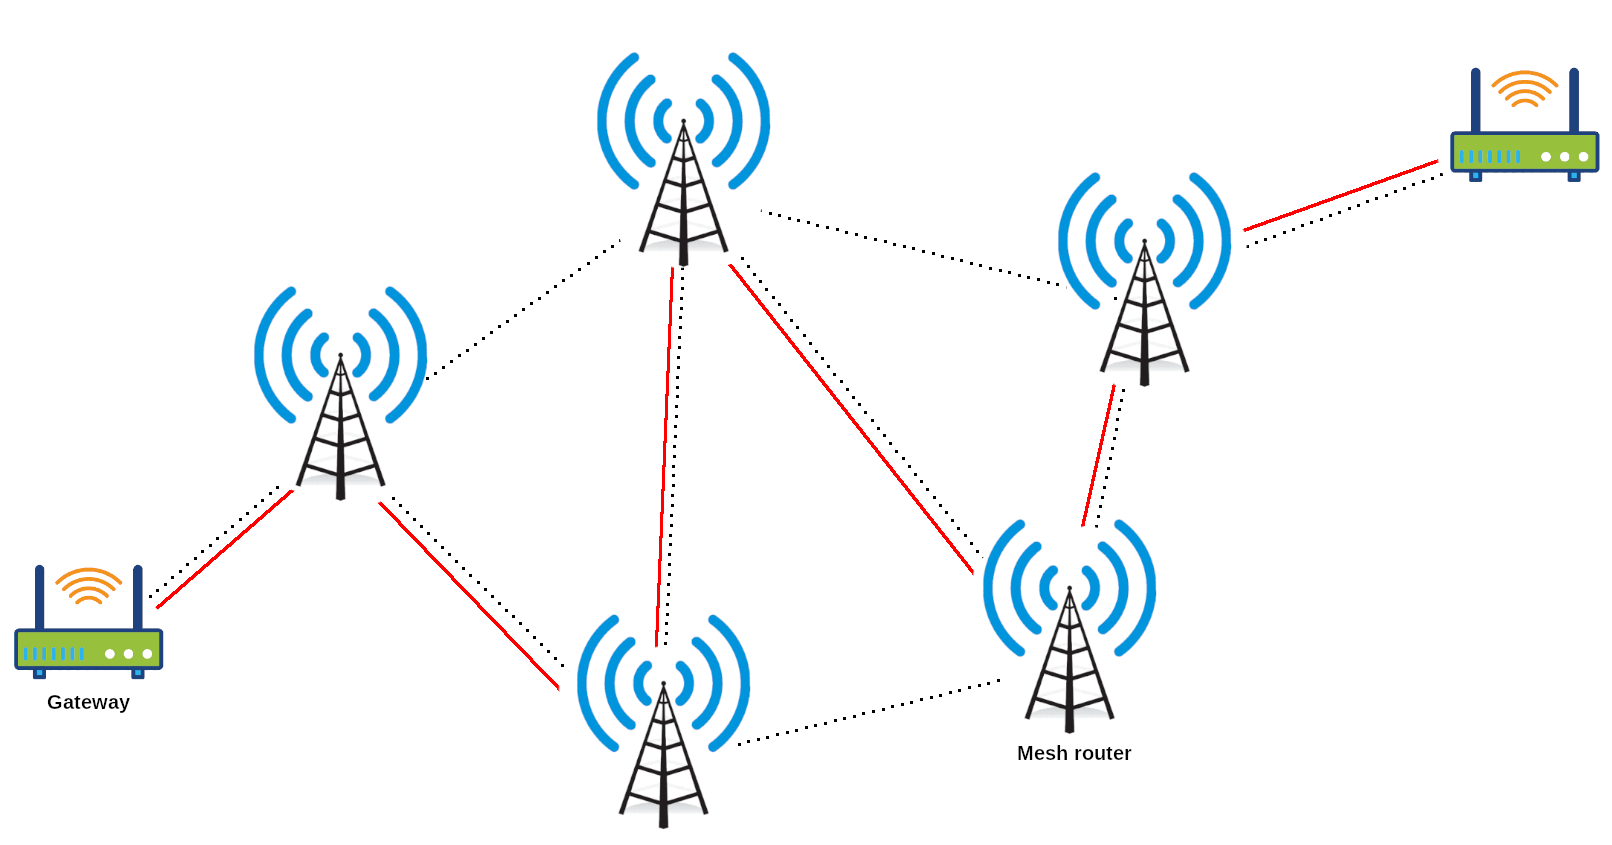
\includegraphics[width=\textwidth]{resources/img/chap4/mesh}
		\caption{Multi-hop network}
		\label{img:multihop}
	\end{figure}
	
	\section{Overview of wireless mesh networks}
		
		% https://beyondroot.com/blog/a-comprehensive-guide-to-mesh-network-in-iot-an-experts-take/		
		With new technologies, such as the ones presented in Section \ref{sec:radio_tech}, wireless mesh networking has been evolving and has reached an ideal point of maturity, which allows it to be useful in the development of IoT devices for mass production.
		Also, the rising number of connected homes and industry support on open-source resources has made mesh networking truly accessible and low-cost.
		Such networks are starting to be regarded as more viable and real choices for commercial as well as industrial IoT applications.
		Besides the possibilities such networks can bring in optimizing communication among nodes, a big advantage is the possibility of bringing connectivity in a system where nodes might have limited connection.
		
		Some of the applications for this network topology are:
		\begin{itemize}
			\item \textit{smart cities}: extending radio signals through campus grounds, business parks, parking garages, and other outdoor facilities;
			\item \textit{healthcare equipment}: monitoring and locating medical equipment, also serve as a backup for medical devices that always require to stay online;
			\item \textit{smart home}: track and manage data from sensors all around the house;
			\item \textit{farming}: in areas where power and connectivity are highly limited, mesh networking is ideal to track sun exposure and water levels across the crops and fields, for example.
		\end{itemize}
	
		Before choosing a mesh network topology it is important to evaluate aspects such as \textit{installation}, \textit{device management} and \textit{support}.
	
		\textit{Energy management} represents an important factor as well, since the connected devices could be small battery operated.
		Thus, efficient transmission techniques and protocols that consider the amount of energy used, must be developed in order to optimally use the batteries on such devices		
		That is why there is a particular network topology, \textit{Low Power Wireless Area Network}, focused on the interconnection of these devices, described in Section \ref{sec:radio_tech}.
		
		Solutions to optimize the networks can be implemented both via hardware, via repeaters, and software.
		% https://ieeexplore.ieee.org/document/4068249
		The latter is mainly implemented with with AI techniques, which allow protocols to ``\textit{learn}'' how to spatially coordinate and adapt contention patterns.
		Authors of \cite{4068249}, for example, have developed new distributed MAC scheduling algorithms by combining synchronous two-level priority RTS/CTS\footnote{ \textit{Request To Send / Clear To Send}} handshaking with randomized time slot selection.
		From these ``\textit{adaptively biasing time-slot selection probabilities based on past history, one can develop variations that are also provably throughput-optimal and exhibit better convergence rates}''.
		
		% https://ieeexplore.ieee.org/document/7968828
		Classic network topologies, such as the ones in Figure~\ref{img:network_topologies}, are not designed for IoT communication and might not be able to meet the requirements for such, and more, dynamic devices, which are also low-powered sensors.
		Another important setback of such networks is their single point of failure nature, which ``\textit{makes the entire system extremely vulnerable when it comes to disasters or even difficult environment as the sensors may need to be deployed into some hardly reachable locations}'' \cite{7968828}.
		
		An example of a multi-hop wireless mesh network is \textit{VANET} (\textit{Vehicular Ad-Hoc Network}), a particular case of wireless multi-hop network, which has the constraint of fast topology changes due to the high node mobility, Figure~\ref{img:vanet}.
		
		\noindent
		\begin{minipage}{0.52\textwidth}
			\begin{figure}[H]
				\centering
				\includegraphics[width=\textwidth]{resources/img/chap4/wms_microsoft}
				\caption[Self organizing wireless mesh networks]{Self organizing wireless mesh networks \cite{bahl2009opportunistic}}
				\label{img:wms_microsoft}
			\end{figure}
		\end{minipage}%
		\hfill%
		\begin{minipage}{0.48\textwidth}\raggedright
			\begin{figure}[H]
				\centering
				\includegraphics[width=\textwidth]{resources/img/chap4/vanet}
				\caption[An example of a VANET]{An example of a VANET \cite{BADIS2015653}}
				\label{img:vanet}
			\end{figure}
		\end{minipage}
		\newline
		
		This is a very important type of network, giving the increasing number of vehicles equipped with computing technologies and wireless communication devices.
		Authors of \cite{BADIS2015653} explain how such increase ``\textit{intervehicle communication is becoming a promising field of research, standardization, and development}''.
		A tangible example can be seen in the rising of electric vehicles and their constant rise in sells on the market, which brought more attention on the aforementioned factors.
		
		Microsoft has also tried to apply mesh networking to normal Internet household use \cite{bahl2009opportunistic}, however, given the improvements in telecommunication infrastructures and the advancement of fiber optics and Internet via cable, the project has been abandoned.
		Their proposed topology is represented in Figure~\ref{img:wms_microsoft}
		This shows how each network topology is better suited for particular scenarios.
		
		Compared to the example of Microsoft's project, a VANET is more suited for a wms since the data transfered among cars is less than the one transfered among houses.
				
		% BLUETOOTH
		% https://www.ericsson.com/en/reports-and-papers/white-papers/bluetooth-mesh-networking
		
		% https://beyondroot.com/blog/a-comprehensive-guide-to-mesh-network-in-iot-an-experts-take/
		The components of a mesh network usually are:
		\begin{itemize}
			\item \textit{nodes}: devices that communicate data with each other;
			\item \textit{gateway}: allows devices to transfer data in the network, also provides a backhaul to the Internet for the local mesh network;
			\item \textit{repeater}: repeaters that maintain signal and forward messages between endpoints
			\item \textit{endpoint}: mesh-only devices that don't route messages for other devices, but send them to other nodes.
		\end{itemize}
		\vspace*{-\baselineskip}
		
		% TODO CHECKED UNTIL HERE
		\subsection{Advantages of WMS}
		
			% https://beyondroot.com/blog/a-comprehensive-guide-to-mesh-network-in-iot-an-experts-take/
			Mesh Network for IoT devices offers enormous benefits that make it sought-after in enterprises and significant in an IoT app development company.
			Self-healing
			
			Like Shortest Path Bridging, Self-healing algorithm automatically chooses the best path to transfer data even if a few nodes lose connection. Specifically, it uses only those connections that are available and working to maintain the task.
			Self-configuring
			
			Due to auto-discovery, mesh networks are self-configuring in nature. Hence, the new nodes calibrate automatically and connect to the network without any previous setup. Consequently, network administration and expansion become easier in mesh networking.
			Scalability and Reliability
			
			In a mesh network, it is way easy to add or remove nodes without any efficiency issue. Usually, issues are in proportion to the devices. However, it is quite the opposite in the case of a mesh network. Adding nodes in a mesh network provides more routes in which data package can travel, which makes the network faster, reliable, and error-resistant.
			Cost Reduction
			
			Since mesh networks do not require internet connection, it consumes ultra-little energy. Meanwhile, sensors are pocket-friendly and long-lasting.
			
			Besides, IoT implementation reduces expenses in many other ways like better management, optimization of resources usage, and more.
		
		\subsection{Disasvantages of WMS}
		
			Drawbacks of Mesh Network in IoT
			
			Though there are ample benefits of a mesh network, it also comes with a few drawbacks. So, it is essential to gain in-depth knowledge of this network before deciding whether a mesh network is a perfect fit for you.
			Low Capacity
			
			Mesh network is the best way of sending small data packages. Unfortunately, it doesn’t perform well while transferring video file sized data.
			
			Still, if transferring a large amount of data is compulsory, then the Wi-Fi mesh network would be a better option.
			Latency
			
			Actively switching from one node to another can decelerate the data receiving process. However, it is not an issue when your system requires a package every few minutes or so. But, it might be not enough for a few systems.
			
			Conversely, a full mesh network can accelerate the data transfer by connecting every node to one another.
			Maintenance
			
			Due to the self-healing ability of the mesh network, finding a non-working node might be time-consuming. Also, we won’t come to know if a node is having an issue.
			
			On the other hand, mesh networks for IoT devices are established to make the IoT system smarter and more efficient. So, the nodes are less prone to crash.
		
			% https://www.inthemesh.com/archive/the-scalability-of-mesh-networks/\\
			
			% https://ieeexplore.ieee.org/document/8071545
			
			% PAPER: LoRaWAN Range Extender for Industrial IoT
	
	\section{Algorithms for lora Wireless Mesh networks}
	
		% https://www.springerprofessional.de/en/research-on-using-the-aodv-protocol-for-a-lora-mesh-network/18715992
	
	\section{Projects}\label{sec:chap4_projects}
		
		Here are three categories of projects:
		
		\subsection{Open source projects}
		
			% https://www.hackster.io/scottpowell69/lora-mesh-chat-5267d9
			\subsubsection{LoRa Mesh Chat}\label{subsubsec:lorameshchat}

				This project consist in an add-on for mobile phones that enable text messaging in a group when outside cellular and Internet coverage.		
					
				\noindent
				\begin{minipage}{0.5\textwidth}% adapt widths of minipages to your needs
					\begin{figure}[H]
						\centering
						\includegraphics[width=.8\textwidth]{resources/img/chap4/lora-mesh-chat-5267d9}
						\caption{ESP32 Lora with OLED}
						\label{img:lora_mesh_chat}
					\end{figure}
				\end{minipage}%
				\hfill%
				\begin{minipage}{0.5\textwidth}\raggedright			
					As explained on the project's webpage \footnotemark, an ESP32 microcontroller with a LoRa antenna and an OLED display is programmed to connect to the phone either via and OTG cable or BLE.
					By using an application on the phone, the user is capable of sending text messages in a group.
				\end{minipage}			
				\footnotetext{{ \url{www.hackster.io/scottpowell69/lora-mesh-chat-5267d9}}}
				
				\subsubsection{Meshtastic}\label{subsubsec:meshtastic}
	
					% https://meshtastic.org/
					% https://github.com/meshtastic
					% https://www.hackster.io/punkgeek/meshtastic-a-hiking-skiing-gps-mesh-communicator-84f999
						
					Meshtastic is an open-source hiking, pilot, skiing, Signal app-extending GPS mesh communicator.
					
					Meshtastic is a project that lets you use inexpensive (\$30 ish) GPS radios as an extensible, super long battery life mesh GPS communicator. These radios are great for hiking, skiing, paragliding - essentially any hobby where you don’t have reliable internet access. Each member of your private mesh can always see the location and distance of all other members and any text messages sent to your group chat.
					
					The radios automatically create a mesh to forward packets as needed, so everyone in the group can receive messages from even the furthest member. The radios will optionally work with your phone, but no phone is required.Our device code is here, our optional Android app is here.
					
					Prebuilt binaries are included on the github sites, but it is quite easy to build from source. Instructions are included in the README. No soldering is required, essentially - buy a \$30 radio and go. We'd love to have your help extending the project - it has been super fun to work on.
		
		\subsection{Research projects}
		
			\subsubsection{Monitoring of Large-Area IoT Sensors Using LoRa Wireless Mesh Network System: Design and Evaluation}
			
			\subsubsection{Black Powder Flow Monitoring in Pipelines by Means of Multi-Hop LoRa Networks}
		
			\subsubsection{Exploring Multi-Hop LoRa for Green Smart Cities}
			
			\subsubsection{Proposal of a Hybrid LoRa Mesh / LoRaWAN Network}
			
			\subsubsection{Beyond the Star of Stars: An Introduction to Multihop and Mesh for LoRa and LoRaWAN}
			
			\subsubsection{LoRa-based Mesh Network for Off-grid Emergency Communications}
			
			% https://ieeexplore.ieee.org/document/9394317
			\subsubsection{LoRaCTP}
			
				a flexible protocol based
				on LoRa technology that allows for the transfer of “content” to
				large distances with very low energy. LoRaCTP provides all the
				necessary mechanisms to make LoRa reliable, by introducing a
				lightweight connection set-up and ideally allowing the sending
				of an as-long-as necessary data message.
			
				\begin{figure}[H]
					\centering
					\includegraphics[width=.75\textwidth]{resources/img/chap4/loractp_packet}
					\caption[Flow of the establishment and interchange of data in LoRaCTP]{Structure of the packet used by the stop-and-wait ARQ. \cite{loractp}}
				\end{figure}
			
				\begin{figure}[H]
					\centering
					\includegraphics[width=.5\textwidth]{resources/img/chap4/loractp_flow}
					\caption[Flow of the establishment and interchange of data in LoRaCTP]{Flow of the establishment and interchange of data in LoRaCTP \cite{loractp}}
				\end{figure}
		
		By content we refer to a self-contained piece of data, like a
		JSON encoded message whose length is in principle unlimited.
		We tested out library with messages of up to 150 kbytes,
		as indicated in Section V. LoRaCTP is based on a unicast
		protocol adopting a classical stop-and-wait ARQ approach
		with a dynamic and adaptive value for the retransmission
		delay. The protocol ensures that information is not lost due to
		dropped packets and that packets are received in the correct
		order.
		
		Each packet is sent by using a three attempts scheme. That
		is, if after three attempts no ACK is received, we suppose
		that the channel is currently busy or too noisy and the content
		sending is dropped.
		
		On top of this flow-control protocol there is a lightweight
		transport protocol that is used to establish a connection be-
		tween a master node, and a client node. Figure 3 shows a sim-
		ple sequence example. Basically the master device “listens”
		to incoming connections. Connections can be established in a
		unicast manner, by providing the address of the master device,
		or using an anycast approach, thus sending to the generic
		“00000000” address and thus receiving the reply from the
		close-by listening device. This possibility allows for a greater
		flexibility in establishing dynamic topologys in rural areas, for
		example.
		
		% https://www.project-owl.com/
		% https://www.reddit.com/r/RTLSDR/comments/bzian5/ltt_showcases_new_lora_mesh_network_devices/

		% TODO DONE CHECK FROM HERE ON
		\subsection{Commercial applications}

			% SONNET
			% https://www.kickstarter.com/projects/sonnet/sonnet-decentralized-mobile-communication
			% https://www.indiegogo.com/projects/sonnet-game-changer-for-wilderness-communications#/
			% GOTENNA
			% https://gotenna.com/
			%				https://gotennamesh.com/products/mesh?utm_source=internal-link&utm_medium=menu&utm_campaign=gotenna.com
			% https://techcrunch.com/2019/06/18/gotenna-is-ramping-up-public-sector-mesh-networking-with-a-24m-c-round/
			\subsubsection{Off grid mesh devices: Sonnet and goTenna}
			
				Both of the following devices use LoRa to create a mesh network and have been designed for emergency off-grid communication, where cellular towers or land-line phones are not physically reachable.
				
				\begin{minipage}{0.38\textwidth}% adapt widths of minipages to your needs
					\begin{figure}[H]
						\centering
						\includegraphics[width=.8\textwidth]{resources/img/chap4/sonnet}
						\caption{Sonnet}
						\label{img:sonnet}
					\end{figure}
				\end{minipage}%
				\hfill%
				\begin{minipage}{0.62\textwidth}\raggedright
					Sonnet\footnotemark, in Figure~\ref{img:sonnet}, connects to the smartphone via Wi-Fi allowing the user to send texts, voice messages, images, data, files and share GPS locations to any other Sonnet users up to several kilometers away, thanks to LoRa.
					This completely removes smartphones' dependency on cellular grid and other network infrastructure, and allows Sonnet to be used even when there is no cellular connectivity or Internet access.
				\end{minipage}		
				\footnotetext{~\url{www.sonnettech.com}}
			
				According to the product's Kickstarter page\footnote{ \url{www.kickstarter.com/profile/sonnet/created}} ``\textit{with Sonnet, data can be relayed up to 16 times to achieve a maximum range of 80 km (50 miles)}''.

				\begin{minipage}{0.5\textwidth}%
					\begin{figure}[H]
						\centering
						\includegraphics[height=6cm]{resources/img/chap4/gotenna}
						\caption{goTenna Mesh}
						\label{img:gotenna}
					\end{figure}
				\end{minipage}%
				\hfill%
				\begin{minipage}{0.5\textwidth}\raggedright
					\begin{figure}[H]
						\centering
						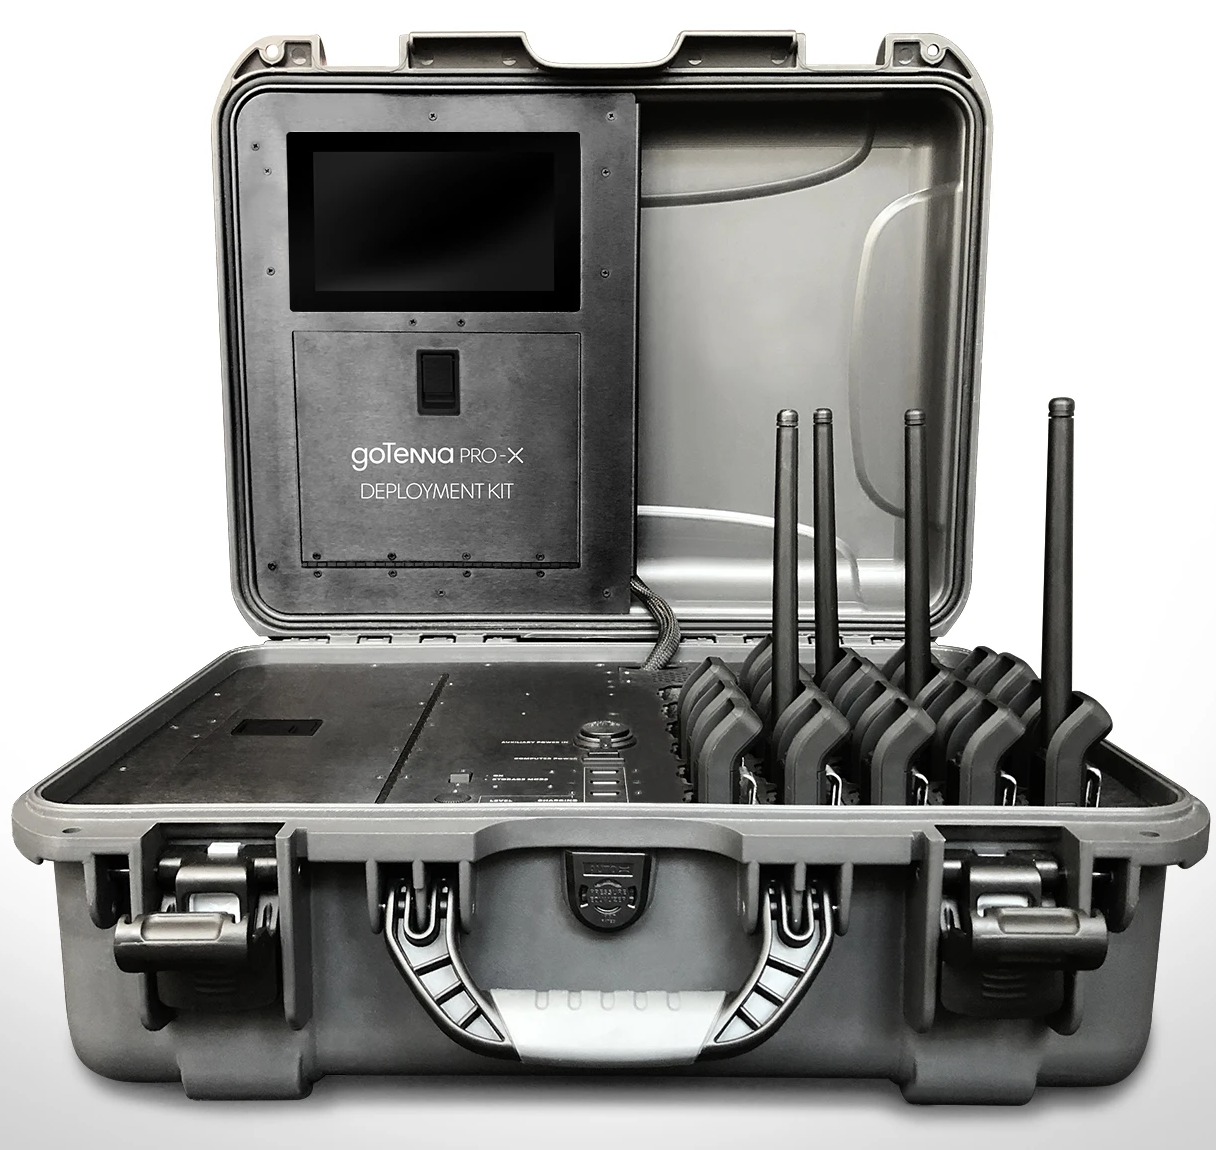
\includegraphics[width=.9\textwidth]{resources/img/chap4/gotenna_prox}
						\caption{goTenna Pro}
						\label{img:gotenna_pro}
					\end{figure}
				\end{minipage}%
				\newpage
				
				The goTenna\footnote{ \url{www.gotenna.com}}, in Figure~\ref{img:gotenna}, offers similar functions as the Sonnet, allowing to send text and GPS locations without the use of a cellphone with Internet connectivity.
				Mesh-networking allows to relay messages from a node to another until they reach destination.
				
				A compact and ruggedized kit, the goTenna Pro X, in Figure~\ref{img:gotenna_pro}, allows control for larger teams that operate in complex environments where it is not possible to be offline.
						
				As Sonnet, goTenna has raised the funds necessary to enter the market as a crowdfunded project on Kickstarter\footnote{ \url{www.kickstarter.com/profile/gotenna/created}}.
				
				Compared to the projects in Section \ref{subsubsec:lorameshchat} and Section \ref{subsubsec:meshtastic}, Sonnet and goTenna offer a more stable network, thanks to the fact that they can be considered finished products which have been thoroughly tested and produced on a bigger scale.
						
			% https://www.linksys.com/us/r/resource-center/whole-home-mesh-Wi-Fi/
			% https://www.pcmag.com/picks/the-best-wi-fi-mesh-network-systems
			\subsubsection{Mesh Wi-Fi}
					
				\textit{Mesh Wi-Fi}, or \textit{Whole Home Wi-Fi} systems, consists of a main router that connects directly to the main modem, and a series of satellite modules, or nodes, placed around the house for full Wi-Fi coverage.
				Each node serves as a hop point for other nodes in the system and are all part of a single wireless network and share the same SSID and password, unlike traditional Wi-Fi routers.
				Weakened signal or Wi-Fi dead spots of the latter are the result of physical obstructions (floor, doors, and walls).
				
				A modular mesh whole home Wi-Fi system is flexible and scalable, giving a customizable method of expanding Wi-Fi coverage without the need to add range extenders, which are certainly effective when it comes to increasing the router range, but they do so at the expense of Wi-Fi performance, which gets cut in half.
			
				\begin{figure}
					\centering
					\includegraphics[width=.9\textwidth]{resources/img/chap4/wifi6}
					\caption{Wi-Fi 6 mesh nodes compared to Wi-Fi range extenders performance}
					\label{img:Wi-Fi6}
				\end{figure}
				
				Wi-Fi 6 is an evolution of 802.11ac technology, which promises increased throughput speeds (up to 9.6Gbps), less network congestion, greater client capacity, and better range performance thanks to the improved wireless technologies, including \textit{Orthogonal Frequency-Division Multiple Access} (\textit{OFDMA}).
				The latter improves overall throughput by breaking Wi-Fi channels into sub-channels, allowing up to 30 users to share a channel at the same time.
				
				Many important manufacturers for network hardware, like Netgear and Cisco, have already implemented such technology and functions in their products available not only for industrial purposes, but also for average users.
				 % Related work
	%!TEX root = ../thesis.tex

% https://en.wikipedia.org/wiki/Kelly_Johnson_(engineer)
% https://en.wikipedia.org/wiki/KISS_principle
\begin{savequote}[40mm]
	\textbf{K}eep\\
	\textbf{I}t\\
	\textbf{S}imple\\
	\textbf{S}tupid
	\qauthor{Kelly Johnson}
\end{savequote}

\chapter{Proposed solution}\label{chapter:proposed_solution}
	
	\textbf{\textcolor{red}{\hl{// To be completed with one or two phrases}}}

	This chapter contains the technical description of the mesh network developed with the FiPy and communicates using LoRa.
	Such mesh network will be referred as ``\textit{Open LoRa Mesh}''.
	Especially such networks is able to accommodate small messages, such as the ones sent by MegaSense, described in Section~\ref{subsec:megasense}.

	Even though it would have been possible to use a simulator, such as ``\textit{The one}''\footnote{ \url{akeranen.github.io/the-one}}, for demonstrating the usefulness of such network, the final project has been realized with Pycom hardware, discussed in Section~\ref{sec:hardware_solution}.
	
%	The code created for this project is open sourced and available on GitHub\footnote{ \url{www.github.com/cipz/OpenLoRaMesh}}.
%	Such code is better explained later in Section~\ref{sec:software_solution} and its subsections.
	
	\section{Network architecture}\label{sec:architecture}
		
		Before talking about the architecture of the mesh, it is important to understand the one of the MegaSense.
		As can be seen in Figure~\ref{img:megasense_architecture}, since each MegaSense device is made to be carried by a person, devices connect each one to the user's phone.
		The latter then communicates with the MegaSense and, via the application developed by the Computer Science Department at the University of Helsinki, sends the air-quality readings and the GPS location, which has been read by the application from the phone itself, to the servers in the cloud.
		
		Communication between MegaSense and phone is done via BLE, and exchanges data such as sensor readings (like NO2,
		O3, CO, battery percentage, \textit{etc.}) and calibration measurements, in \texttt{JSON} format.
		Thus each device has to be linked to a person's phone, which might enhance the portability of the device, but not its possibility to read data independently if placed in a specific location.
		
		\begin{figure}[h]
			\centering
			\includegraphics[width=.75\textwidth]{resources/img/chap5/architecture_megasense}
			\caption{MegaSense architecture}
			\label{img:megasense_architecture}
		\end{figure}
	
		One of the goals Open LoRa Mesh tries to achieve, is to give independence to these devices, so that they can communicate one another and allow information to be passed along between nodes without the aid of a user's phone.
	
		This is why the architecture would evolve from the one in Figure~\ref{img:megasense_architecture} to Figure~\ref{img:openmesh_architecture}: the phone is replaced by a FiPy, which also connects to the MegaSense via BLE, and sends the data acquired from the sensors in the network.
		Nodes communicate with each other via LoRa, detailed in Section~\ref{subsec:lora_lorawan}, and exchange data using mainly \textit{LoRaCTP}, described in Section~\ref{subsec:loractp}.
		
		\begin{figure}[h]
			\centering
			\includegraphics[width=.7\textwidth]{resources/img/chap5/mesh-architecture-1}
			\caption{Open LoRa Mesh architecture}
			\label{img:openmesh_architecture}
		\end{figure}
		
		Each FiPy board represents a node on the network, which in this case is a ``\textit{Flat Wireless Mesh}'', where each node acts both as data provider and as data forwarder.
		Although simple, such network architecture is well known from the previously mentioned, Section~\ref{sec:scalability}, Gupta and Kumar \cite{825799}.
		Besides not scaling well and having the potential to put very high resource constraints, ``\textit{addressing schemes and service discovery would prove to be a major bottleneck against scalability}'' \cite{92000412}.

	\section{Open LoRa Mesh Hardware}\label{sec:hardware_solution}
	
		For the development of Open LoRa Mesh, the chosen hardware to replace the phone in the original MegaSense architecture is composed by Pycom's FiPy microcontrollers, along with its shields, like the PyTrack and the PySense.
		A prototype of the MegaSense device was also given from the developers of the project in order to test the connectivity with the Pycom boards and test its capacity to send and receive data from other nodes in the network.
		All devices can be seen together in Figure~\ref{img:irl_picture_1}.
		
		\begin{figure}[h]
			\centering
			\includegraphics[width=\textwidth]{resources/img/chap5/mesh-irl-picture}
			\caption{FiPy with PyTrack, LoRa antenna, GPS antenna and MegaSense prototype}
			\label{img:irl_picture_1}
		\end{figure}
		
		Although the expansion board is important, the FiPy is the one that contains all the chips that allow connectivity, as said in Section~\ref{sec:pycom}.
		After an initial evaluation on the requirements necessary in creating a network for exchanging messages among air quality sensing devices, Pycom's boards have come first considering the numerous possibilities it allows for prototyping.
		
		The exact hardware with which this project has been completed is: four FiPy boards, one PyTrack 2X, one PyTrack, two PySense shields and one MegaSense prototype, Figure~\ref{img:megasense_picture}.
		Pycom boards do not have a USB connection directly on them, so they can be programmed either using a shield or via an UART (Universal Asynchronous Receiver-Transmitter) to USB.
		
		Alternative microcontrollers, such as the Raspberry Pi Pico, Raspberry Pi 4, Arduino Nano 33 BLE Sense, and ESP32 boards have been discard given either their excessive power or their need for multiple expansion shields.
				
	\section{Open LoRa Mesh Software}\label{sec:software_solution}
	
		While the Arduino's C++ dialect divides the code in two main functions, the \texttt{setup()} and \texttt{loop()}, as mentioned in Chapter~\ref{chapter:technologies}, the Pycom boards use two files to separate an initial bootstrap of the board and a main section of the code.
		These two special files are called \texttt{boot.py} and \texttt{main.py} respectively.
		
		The following section explains the addressing scheme in LoRa, which is important to understand.
		Afterwards, the algorithms made for this project are delineated and it is shown how they have been implemented.
		
		The FiPy boards have been programmed using Micropython, and the firmware flashed on the boards, at the time of writing, is \texttt{v1.16.5}.
		
		\subsection{LoRa addressing scheme}\label{subsec:lora_addressing}
		
			\textbf{\textcolor{red}{\hl{// To be completed}}}
		
			% Hardware Addressing Schemes
		
		
			%calcolare transmission times
		
%		\newpage\phantom{blabla}
%		\newpage\phantom{blabla}
%		\newpage\phantom{blabla}
%		\newpage\phantom{blabla}	
		
		\subsection{Algorithms}\label{subsec:algorithms}
	
			% DRAWING AUTOMATA
			% https://latexdraw.com/automata-diagrams-in-latex/
			% https://hayesall.com/blog/latex-automata/
			
			% DRAWING FLOWCHART
			% https://www.overleaf.com/learn/latex/LaTeX_Graphics_using_TikZ%3A_A_Tutorial_for_Beginners_(Part_3)%E2%80%94Creating_Flowcharts

			This section shows in depth how the software works: for each significant building block of the code there are flowcharts and finite-state automata (or FSA).
			The flowcharts describe the algorithms and show what functions are called, while finite-state machines show what states the devices can be in and how they arrive in such states.
			% Note: automata is plural
			For a graphical reason, each state of the following automata is abbreviated, and the full state is described in a table underneath it.
			
			Such vision should allow to understand the system from a broader point of view to a more detailed one, where every function is analyzed.
			
			\subsubsection{Overview of the whole system}
			
				As previously said, the FiPy is divided in two files, \texttt{boot.py} and \texttt{main.py}.
				
%				\begin{figure}[h]
%					\centering
%					\begin{tikzpicture}[shorten >=1pt,node distance=2cm,on grid,auto]
%					
%					% Help grid
%					% \draw [help lines] (-1,1) grid (6,-6);
%					
%					\tikzstyle{every state}=[fill={rgb:black,1;white,5}]
%					
%					
%					\node[state, initial]  			(s_0)                 	{$s_0$}; % START
%					\node[state] 					(s_1)	[right of=s_0]	{$s_1$}; % BOOT
%					\node[state, accepting]			(s_2) 	[above right of=s_1]	{$s_2$}; % MAIN LOOP
%					\node[state, accepting]			(s_3) 	[below right of=s_1]	{$s_3$}; % LISTENER LOOP
%					
%					\path[->]
%					(s_0) edge node {} (s_1)
%					(s_1) edge node {} (s_2)
%					(s_3) edge node {} (s_1)
%					(s_2) edge [loop right] node {} ()
%					(s_3) edge [loop right] node {} ();
%					
%					\end{tikzpicture}
%					\caption{FSA for the overview of the whole system}
%					\label{img:fsa_overview}
%				\end{figure}
%			
%				\begin{table}[h]
%					\begin{center}
%						\begin{tabularx}{0.85\textwidth}{@{}|Y|Y|Y|@{}} 
%							\hline
%							State abbreviation & Full state name & State description \\\hline
%							$start$ && \\\hline
%							$s_{0}$ && \\\hline
%							$s_{1}$ && \\\hline
%							$s_{2}$ && \\\hline
%							$s_{3}$ && \\\hline
%						\end{tabularx}
%						\caption{Main algorithm fsm description}
%						\label{table:fsm_main}
%					\end{center}
%				\end{table}
%			
%				\begin{figure}
%					\centering
%					\tikzstyle{startstop} = [rectangle, rounded corners, minimum width=3cm, minimum height=1cm,text centered, draw=black, fill=red!30]
%					\tikzstyle{io} = [trapezium, trapezium left angle=70, trapezium right angle=110, minimum width=3cm, minimum height=1cm, text centered, draw=black, fill=blue!30]
%					\tikzstyle{process} = [rectangle, minimum width=3cm, minimum height=1cm, text centered, draw=black, fill=orange!30]
%					\tikzstyle{decision} = [diamond, minimum width=3cm, minimum height=1cm, text centered, draw=black, fill=green!30]
%					\tikzstyle{arrow} = [thick,->,>=stealth]
%					\begin{tikzpicture}[node distance=2cm]
%						\node (start) [startstop] {Start};
%						\node (in1) [io, below of=start] {Input};
%						\node (pro1) [process, below of=in1] {Process 1};
%						\node (dec1) [decision, below of=pro1] {Decision 1};
%						\node (pro2a) [process, below of=dec1, yshift=-0.5cm] {Process 2a};
%						\node (pro2b) [process, right of=dec1, xshift=2cm] {Process 2b};
%						\node (out1) [io, below of=pro2a] {Output};
%						\node (stop) [startstop, below of=out1] {Stop};
%
%					\end{tikzpicture}
%				\end{figure}
%				
%				\begin{figure}
%					\centering
%					
%					% BLOCK STYLES
%					\tikzstyle{decision} = [diamond, draw, fill=blue!20, text width=4.5em, text badly centered, node distance=3cm, inner sep=0pt]
%					\tikzstyle{block} = [rectangle, draw, fill=blue!20,	text width=4em, text centered, rounded corners, minimum height=3em]
%					\tikzstyle{line} = [draw, -latex']
%					\tikzstyle{cloud} = [draw, ellipse,fill=red!20, minimum height=2.5em, minimum width=3.5em]
%					
%					\begin{tikzpicture}[node distance = 2cm, auto]
%					
%					% BLOCKS
%					
%					\node [cloud] 							(start) 	{start};
%					\node [block, below of=start] 	 		(boot) 		{boot()};
%					\node [block, below left  of=boot] 		(main) 		{main()};
%					\node [block, below right of=boot] 		(listen) 	{listen()};
%					\node [cloud, below right of=main] 		(end) 		{end};
%					
%					% EDGES
%					\path [line] (start) -- (boot);
%					\path [line] (boot) -- (main);
%					\path [line] (main) -- (end);
%					\path [line] (boot) -- (listen);
%					\path [line] (listen) -- (end);
%					
%					\end{tikzpicture}
%					\caption{test}
%					\label{test}
%				\end{figure}
			
			\subsubsection{Boot}
			
			\subsubsection{Main}
			
			\subsubsection{Plain listener}
	
			\subsubsection{Mesh initiation}
			
			\subsubsection{Broadcast mesh information}
			
%				\begin{figure}[h]
%					\centering
%					\includegraphics[width=.7\textwidth]{resources/img/chap5/message_exchange}
%					\caption{``\textit{Open LoRa Mesh}'' architecture}
%					\label{img:openmesh_architecture}
%				\end{figure}
			
			\subsubsection{Loop}
			
			\subsubsection{Listen}
			
			\subsubsection{Message forwarding}
			
			\subsubsection{MegaSense communication}
			
			\subsubsection{Message transmission}
			
		\subsection{Supported messages}
		
	\section{Other files}
	
%		\begin{figure}[h]
%			\centering
%			\includegraphics[width=.5\textwidth]{resources/img/chap5/tree_files}
%			\caption{List of files that compose the Open LoRa Mesh project}
%			\label{img:files}
%		\end{figure}
		
	\section{Microcontroller sleep cycle}\label{sec:sleep}
	
		Most IoT devices that compose LPWANs have three main modes, or profiles: \textit{sense}, \textit{connect} and \textit{sleep}.
		Sense and connect refer respectively to gathering data from the sensors and sending it into the network, while sleep refers to a sleep-mode energy consumption where most processes in the device are halted, and some circuits may be powered down.
		It can be considered a design trade-off between functionality, size, and battery lifetime.
		
		This energy consumption profile is important because it helps maximizing the battery life, which currently is one of the most considerable bottlenecks in IoT low-power devices, as explained in Section~\ref{sec:trends}.
		
		However, in the implementation of the Open LoRa Mesh, nodes do not have such functionality implemented, since might it be the cause for network disruptions.
		
		For example, if a new node might want to join a network, but the nearest physical node is in sleep mode, there would be no possibility for the new node to request data about the network, thus wasting time and resources while waiting to the other node to come back online.
		
		Such mode could be implemented but would require an careful analysis on the evolution of the network in time, also would require a network made entirely, or mostly of static nodes.
		This thought is reviewed again in Section~\ref{sec:software_improvements}.
			
	\section{Use cases}
		
		\subsection{Mobile network}
		
			e.g. in a bike sharing environment
		
		\subsection{Fixed network}
		
			e.g. in a monitoring values of air quality inside a building
		
		\subsection{Hybrid network}
		
			e.g. integrating mobile sensors given to users with a network of fixed sensors % Proposed solution
 	%!TEX root = ../thesis.tex

\begin{savequote}[60mm]
	There's no reason to have a plan B\\
	because it distracts from plan A.
	\qauthor{Will Smith}
\end{savequote}

\chapter{Results and experimentation}\label{chapter:results}
	
	This chapter expands the previous one by verifying the usability of the Open LoRa Mesh.
	Particularly describes some test scenarios in which Open LoRa Mesh has been set up in order to record its performances.
	
	\section{Experiments}
	
		\subsection{Mesh creation}
		
		\subsection{Node addition}

		\subsection{Node removal}
		
		\subsection{Message propagation}
		
		\subsection{LoRa reach}
	
	\section{Results} % Results and experimentation
	%!TEX root = ../thesis.tex

\begin{savequote}[70mm]
	Be fearful when others are greedy,\\
	and greedy when others are fearful.
	\qauthor{Warren Buffet}
\end{savequote}

\chapter{Conclusions}\label{chapter:conclusions}

	Mesh networks are ``\textit{decentralized, easy to deploy, and characterized by dynamic self-organization, self-configuration, and self-healing properties}'' \cite{Sampaio-2015}.
	Such properties enable fast deployment, low installation cost, and reliable communication.
	
	This thesis describes an implementation of a mesh network solution for IoT devices, particularly for an air quality sensing device: MegaSense, described in Section \ref{subsec:megasense}.
	
%	This project represents
%	
%	It has been implemented on pycom hardware, the software is available on github in 
	
	Besides summarizing the previously discussed arguments, this chapter contains some personal considerations by the author.

	\section{Contributions}
	
		\textbf{\textcolor{red}{\hl{// To be completed}}}

	\section{Future work}
		
		\textbf{\textcolor{red}{\hl{// To be completed}}}
	
		\subsection{Hardware improvements}
			
%			Note from the author, it must be taken in consideration that the device can run hot, an application of the device such as on a bike that is parked out in the sun may overheat the device.
%			On pycom's documentation it is written that the fipy can support temperatures up to x
%			Thus an interesting improvement could be to add a heatsink in order to lower the temperatures and improve the lifespan of the device
		
			\textbf{\textcolor{red}{\hl{// To be completed}}}

		\subsection{Software improvements}
		
%			Better logging 
%			
%			improvement on routing table and algorithm used for message forwarding 

			\textbf{\textcolor{red}{\hl{// To be completed}}}

	\section{Personal considerations}
	
		\subsection{About the Pycom boards}\label{sec:working_with_pycom}
		
			Compared to working with other boards, such as the Arduino, Pycom boards are more complete, since they offer better specifications, for both computing power and memory, connectivity and support.
			
			For prototyping, Arduino boards offer very good opportunities and have been on the market for a longer time, allowing consumers to get acquainted and know the brand.
			% https://patentlyo.com/patent/2011/01/tracing-the-quote-everything-that-can-be-invented-has-been-invented.html
			Sometimes, working with Arduino feels like ``\textit{everything that can be invented has been invented}'', as said by Charles H. Duell, since there is so many people who have made all kind of projects and are sharing them online.
			
			The FiPy, on the other hand, would offer more stability and 
			
			An example where the FiPy would offer a great improvement over an Arduino board would be this smart home application\footnote{ \url{www.instructables.com/Smart-Home-With-Arduino-Ethernet-Shield-and-Teledu}}.
			Such project contains an Arduino Mega board with various sensors and relays, all connected via a specifically build website, with the use of a third-party API handler for the Arduino.
			The Arduino connects to the Internet via an Ethernet shield, thus sends data by cable.
			A FiPy would allow a smaller footprint and no need for a shield, besides avoiding the use of a third-party API handler.
			
			It can easily become hard to create a project with a messed up codebase if not kept organized from the beginning.
			Even if this is true for all software projects, it is particularly easy to achieve when dealing with microcontrollers, which have limitations on computation and memory, as explained in Chap. \ref{chapter:technologies}.
			
		\subsection{About mesh networking}\label{sec:mesh_considerations}
		
			As said in Chapter \ref{chapter:technologies}, each network topology is better suited for particular scenarios.
			It is not possible to have a ``\textit{one size fits all}'' network for all possible applications that need to exchange data.
			As for all questions in computer science, the answer to the question where a mesh network is useful is ``\textit{it depends}''.
			
			Mesh networking is a very interesting network topology which, compared to all the others in Figure~\ref{img:network_topologies}, has still a lot of research possibilities.
			In conjunction with AI and machine learning, it is possible to achieve an optimal level of connectivity in such networks.
			The bottlenecks would then be represented by the computing power in the nodes, and in the algorithm used in case one of the nodes fail, or new nodes are added into the network.

			Scalability of such networks, as spoken about in Section \ref{sec:scalability}, is a very interesting research scenario since it is one of the major deciding elements for any new networking technology to be accepted.
			Factors such as multi-hopping, protocol overhead, and wireless interference limit the scalability of such networks.
			Mesh networks will be more and more common, but I believe they will be used in conjunctions with other topologies: for example a local mesh network that allows communication between sensors in a house and a gateway node interacts with other networks in a different topology.
			
			Security is another important factor when considering in mesh networking.
			Since each node receives and analyzes packages, there is no totally effective solution for a secure network.
			Adding security features such as encryption/decryption algorithms and other checks, would result in a big overhead on small IoT devices.
			Also, like other radio technologies, anyone can read messages, encrypted or not, ``\textit{flying}'' through the air.
	
	%!TEX root = ../thesis.tex

\renewcommand\thechapter{A}
\chapter{Appendix A}\label{ch:AppendixA}
	
	\lipsum[1-2] % Programming pycom's FiPy and PyTrack
	%!TEX root = ../thesis.tex

\renewcommand\thechapter{B}
\chapter{Techinical Manual}\label{ch:AppendixB}

 % Glossary of terms and abbreviations
	
	\addcontentsline{toc}{chapter}{Acknowledgments}
	\acknowledgments
	
	\cleardoublepage
	\phantomsection
	
	\addcontentsline{toc}{chapter}{References}
	\bibliography{references}
	
	\cleardoublepage
	\phantomsection
	
	\addcontentsline{toc}{chapter}{Glossary}
	\printglossary

	\backmatter

\end{document}